\chapter{Combinatorics of multiple braid arrangements}
\label{part:multiBraidArrangements}

In this first part, we study the combinatorics of hyperplane arrangements obtained as unions of generically translated copies of the braid arrangement.
In \cref{sec:arrangements}, we first recall some classical facts on the enumeration of hyperplane arrangements (\cref{subsec:arrangements}), present the classical braid arrangement (\cref{subsec:braidArrangement}), and define our multiple braid arrangements (\cref{subsec:multiBraidArrangement}).
Then in \cref{sec:flatPoset}, we describe their flat posets in terms of partition forests (\cref{subsec:partitionForests}) and rainbow forests (\cref{subsec:rainbowForests}), from which we derive their M\"obius polynomials (\cref{subsec:MobiusPolynomialMultiBraidArrangement}), and some surprising formulas for their numbers of vertices (\cref{subsec:verticesMultiBraidArrangement}) and regions (\cref{subsec:regionsMultiBraidArrangement}).
Finally, in \cref{sec:facePoset}, we describe their face posets in terms of ordered partition forests (\cref{subsec:orderedPartitionForests}), and explore some combinatorial criteria to describe the ordered partition forests that appear as faces of a given multiple braid arrangement (\cref{subsec:PFtoOPF,subsec:criterionOPF}).

%%%%%%%%%%%%%%%%%%%%%%%%%%%%%%%%%%%%%%

\section{Recollection on hyperplane arrangements and braid arrangements}
\label{sec:arrangements}

%%%%%%%%%%%%%%%

\subsection{Hyperplane arrangements}
\label{subsec:arrangements}

We first briefly recall classical results on the combinatorics of affine hyperplane arrangements, in particular the enumerative connection between their intersection posets and their face lattices due to T.~Zaslavsky~\cite{Zaslavsky}.

\begin{definition}
A finite affine real \defn{hyperplane arrangement} is a finite set~$\arrangement$ of affine hyperplanes in~$\R^d$.
\end{definition}

\begin{definition}
A \defn{region} of~$\arrangement$ is a connected component of~$\R^d \ssm \bigcup_{H \in \arrangement} H$.
The \defn{faces} of~$\arrangement$ are the closures of the regions of~$\arrangement$ and all their intersections with a hyperplane of~$\arrangement$.
The \defn{face poset} of~$\arrangement$ is the poset~$\facePoset$ of faces of~$\arrangement$ ordered by inclusion.
The \defn{$f$-polynomial}~$\fPol$ and \defn{$b$-polynomial}~$\bPol$ of~$\arrangement$ are the polynomials
\[
\fPol \eqdef \sum_{k = 0}^d f_k(\arrangement) \, x^k
\qquad\text{and}\qquad
\bPol \eqdef \sum_{k = 0}^d b_k(\arrangement) \, x^k ,
\]
where~$f_k(\arrangement)$ denotes the number of $k$-dimensional faces of~$\arrangement$, while~$b_k(\arrangement)$ denotes the number of bounded $k$-dimensional faces of~$\arrangement$.
\end{definition}

\begin{definition}
A \defn{flat} of~$\arrangement$ is a non-empty affine subspace of~$\R^d$ that can be obtained as the intersection of some hyperplanes of~$\arrangement$.
The \defn{flat poset} of~$\arrangement$ is the poset~$\flatPoset$ of flats of~$\arrangement$ ordered by reverse inclusion.
\end{definition}

\begin{definition}
\label{def:MobiusPolynomial}
The \defn{M\"obius polynomial}~$\mu_{\arrangement}(x,y)$ of~$\arrangement$ is the polynomial defined by
\[
\mobPol \eqdef \sum_{F \le G} \mu_{\flatPoset}(F,G) \, x^{\dim(F)} \, y^{\dim(G)},
\]
where~$F \le G$ ranges over all intervals of the flat poset~$\flatPoset$, and~$\mu_{\flatPoset}(F,G)$ denotes the \defn{M\"obius function} on the flat poset~$\flatPoset$ defined as usual by
\[
\mu_{\flatPoset}(F, F) = 1
\qquad\text{and}\qquad
\sum_{F \le G \le H} \mu_{\flatPoset}(F,G) = 0
\]
for all~$F < H$ in~$\flatPoset$.
\end{definition}

\begin{remark}
Our definition of the M\"obius polynomial slightly differs from that of~\cite{Zaslavsky} as we use the dimension of~$F$ instead of its codimension, in order to simplify slightly the following statement.
\end{remark}

\begin{theorem}[{\cite[Thm.~A]{Zaslavsky}}]
\label{thm:Zaslavsky}
The $f$-polynomial, the $b$-polynomial, and the M\"obius polynomial of the hyperplane arrangement~$\arrangement$ are related by
\[
\fPol = \mobPol[\arrangement][-x][-1]
\qquad\text{and}\qquad
\bPol = \mobPol[\arrangement][-x][1].
\]
\end{theorem}

\begin{example}
%
\begin{figure}
%	\begin{overpic}[scale=.9]{intersectionPoset}
%		\put(72.5, -2){$1$}
%		\put(51, 10){$-1$}
%		\put(61, 10){$-1$}
%		\put(71, 10){$-1$}
%		\put(82, 10){$-1$}
%		\put(94, 10){$-1$}
%		\put(51.5, 32){$2$}
%		\put(66, 32){$1$}
%		\put(80, 32){$1$}
%		\put(93.5, 32){$2$}
%	\end{overpic}
%	\caption{A hyperplane arrangement (left) and its intersection poset with its M\"obius function (right).}
	\centerline{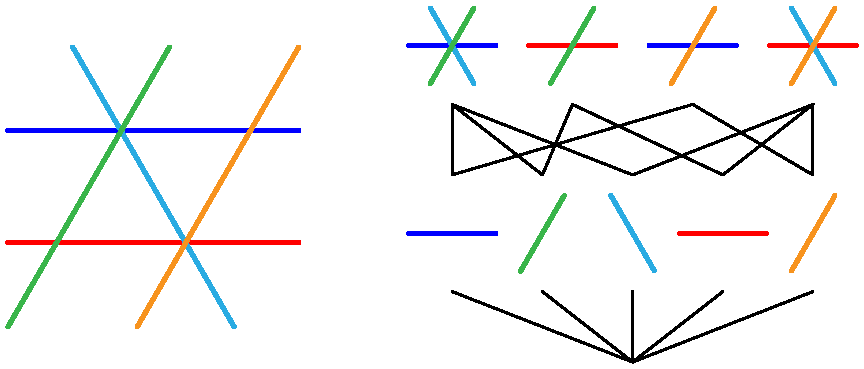
\includegraphics[scale=.9]{intersectionPoset}}
	\caption{A hyperplane arrangement (left) and its intersection poset (right).}
	\label{fig:arrangement}
\end{figure}
%
For the arrangement~$\arrangement$ of $5$ hyperplanes of \cref{fig:arrangement}, we have
\[
\mobPol = x^2y^2 - 5x^2y + 6x^2 + 5xy - 10x + 4 ,
\]
so that
\[
\fPol = \mobPol[\arrangement][-x][-1] = 12 \, x^2 + 15 \, x + 4 
\qquad \text{and}\qquad
\bPol = \mobPol[\arrangement][-x][1] = 2 \, x^2 + 5 \, x + 4 .
\]
\end{example}

\begin{remark}
\label{rem:characteristicPolynomial}
The coefficient of~$x^d$ in the M\"obius polynomial~$\mobPol$ gives the more classical \defn{characteristic polynomial}
\[
\charPol \eqdef [x^d] \, \mobPol = \sum_F \mu_{\flatPoset}(\R^d,F) \, y^{\dim(F)} .
\]
By \cref{thm:Zaslavsky}, we thus have
\[
f_d(\arrangement) = (-1)^d \, \charPol[\arrangement][-1] 
\qquad\text{and}\qquad
b_d(\arrangement) = (-1)^d \, \charPol[\arrangement][1].
\]
\end{remark}

%%%%%%%%%%%%%%%

\subsection{The braid arrangement}
\label{subsec:braidArrangement}

We now briefly recall the classical combinatorics of the braid arrangement.
See \cref{fig:facePosetBraidArrangement3,fig:intersectionPosetBraidArrangement3,fig:intersectionPosetBraidArrangement4} for illustrations when~$n = 3$ and~$n = 4$.

%\begin{figure}
%	\centerline{\includegraphics[scale=.9]{figures/intersectionPosetBraidArrangement3Full}}
%	\caption{The braid arrangement $\braidArrangement[3]$ (left), its flat poset~$\flatPoset[{\braidArrangement[3]}]$ (middle), and the partition poset~$\partitionPoset[3]$ (right).}
%	\label{fig:braidArrangement3}
%\end{figure}

\afterpage{
\begin{figure}
	\centerline{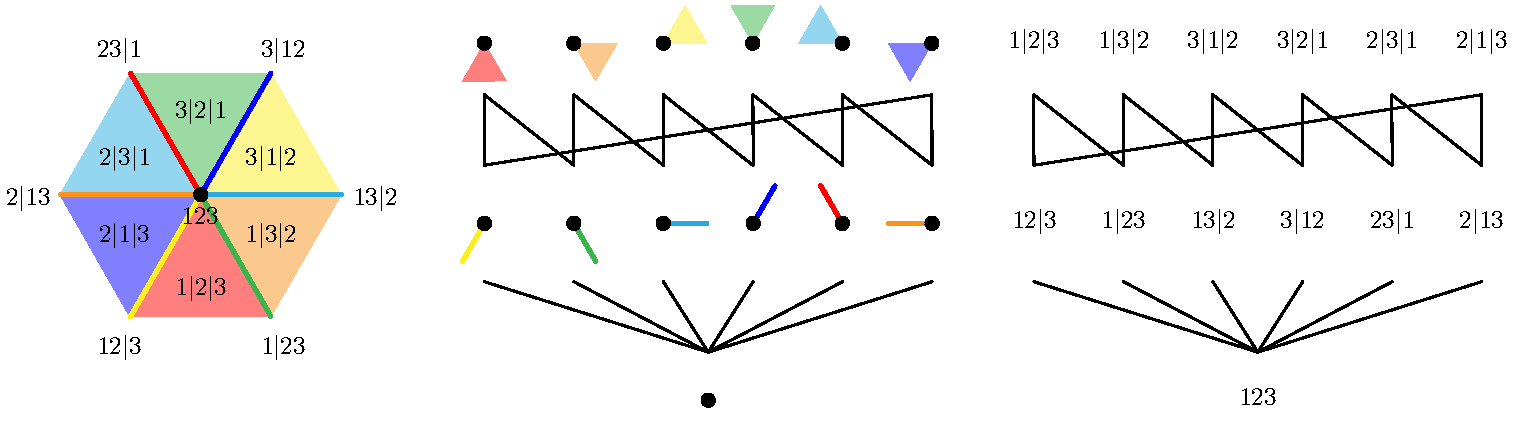
\includegraphics[scale=.6]{figures/facePosetBraidArrangement3}}
	\caption{The face poset~$\facePoset[{\braidArrangement[3]}]$ of the braid arrangement $\braidArrangement[3]$ (left), where faces are represented as cones (middle) or as ordered set partitions of~$[3]$ (right).}
	\label{fig:facePosetBraidArrangement3}
\end{figure}
}

\afterpage{
\begin{figure}
	\centerline{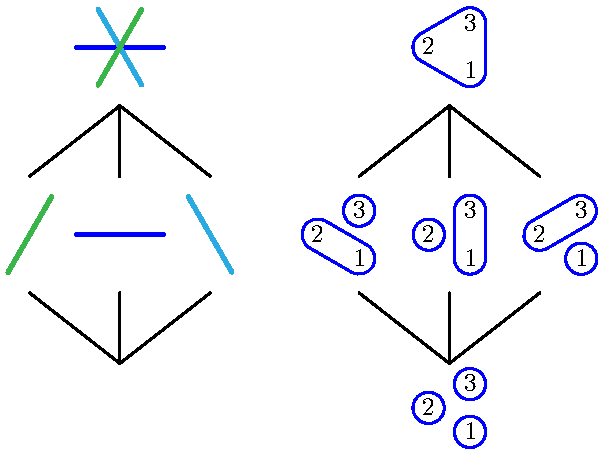
\includegraphics[scale=.6]{figures/intersectionPosetBraidArrangement3}}
	\caption{The flat poset~$\flatPoset[{\braidArrangement[3]}]$ of the braid arrangement $\braidArrangement[3]$, where flats are represented as intersections of hyperplanes (left) or as set partitions of~$[3]$ (right).}
	\label{fig:intersectionPosetBraidArrangement3}
\end{figure}
}

\afterpage{
\begin{figure}
	\centerline{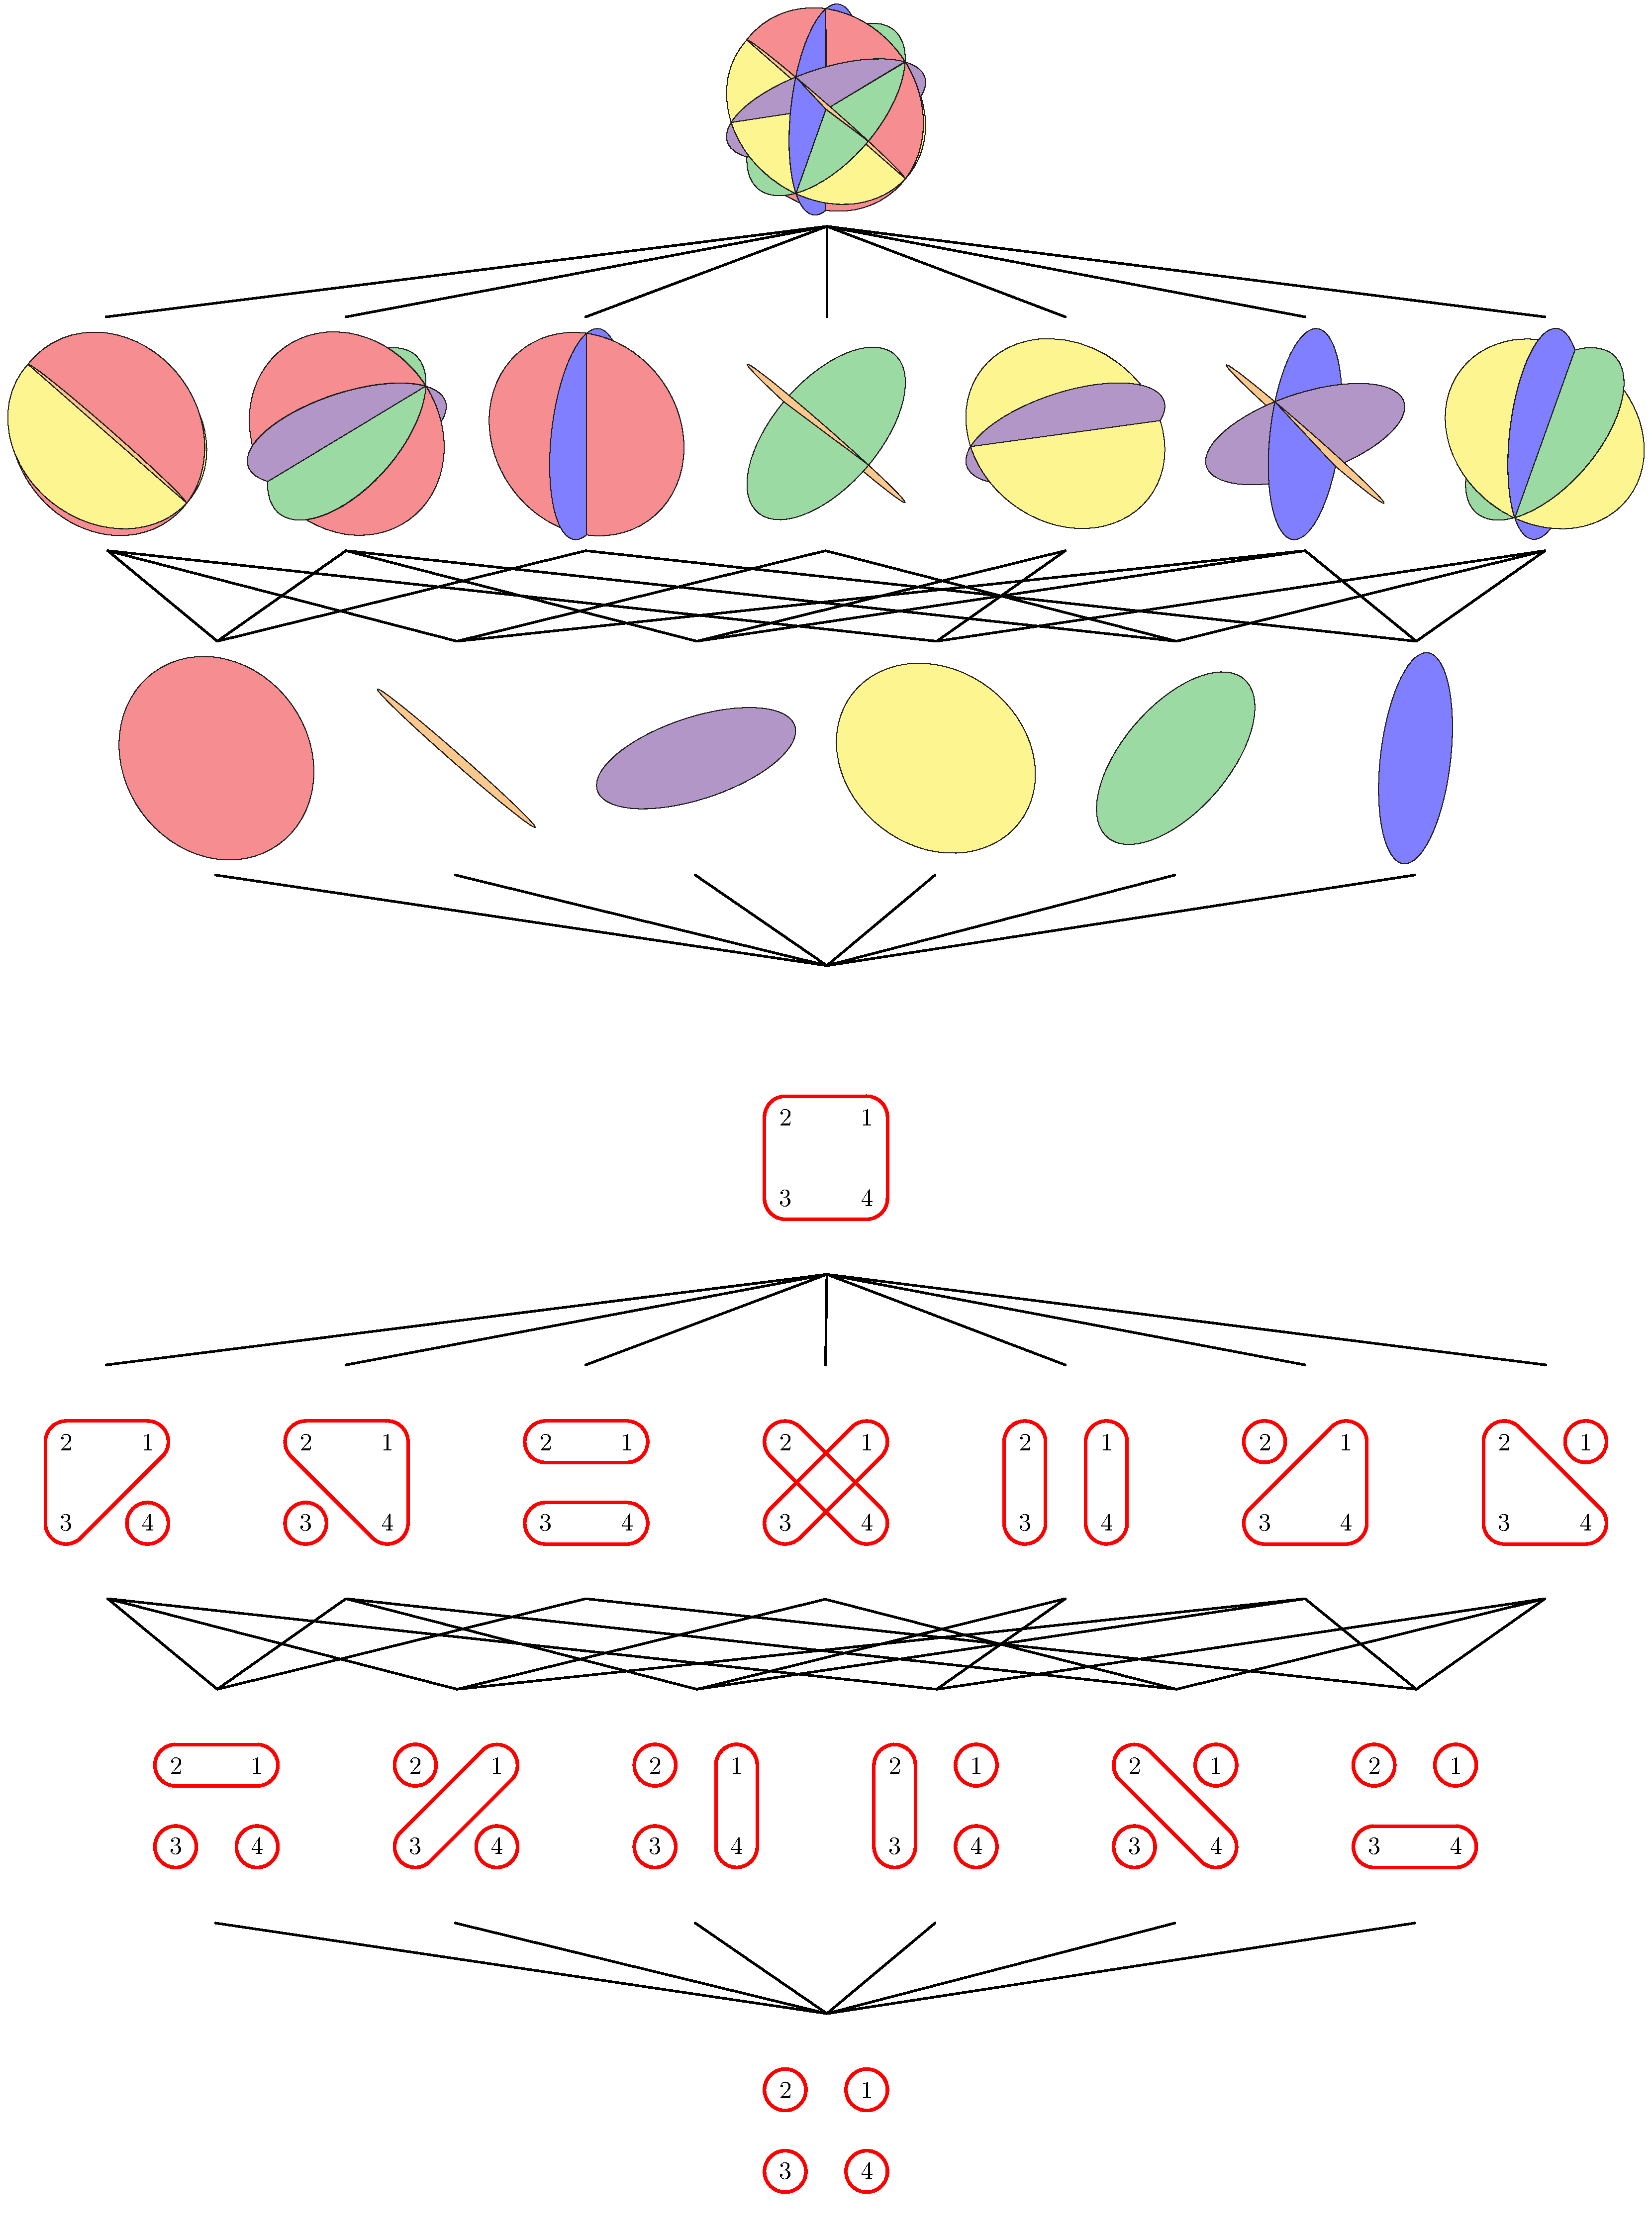
\includegraphics[scale=.26]{figures/intersectionPosetBraidArrangement4}}
	\caption{The flat poset~$\flatPoset[{\braidArrangement[4]}]$ of the braid arrangement $\braidArrangement[4]$, where flats are represented as intersections of hyperplanes (top) or as set partitions of~$[4]$ (bottom).}
	\label{fig:intersectionPosetBraidArrangement4}
\end{figure}
}

\begin{definition}
Fix~$n \ge 1$ and denote by~$\HH$ the hyperplane of~$\R^n$ defined by~$\sum_{s \in [n]} x_s = 0$.
The \defn{braid arrangement}~$\braidArrangement$ is the arrangement of the hyperplanes~$\set{\b{x} \in \HH}{x_s = x_t}$ for all~${1 \le s < t \le n}$.
\end{definition}

\begin{remark}
\label{rem:essential}
Note that we have decided to work in the space~$\HH$ rather than in the space~$\R^n$.
The advantage is that the braid arrangement~$\braidArrangement$ in~$\HH$ is essential, so that we can speak of its rays.
Working in~$\R^n$ would change rays to walls, and would multiply all M\"obius polynomials by a factor~$xy$.
\end{remark}

The combinatorics of the braid arrangement~$\braidArrangement$ is well-known.
The descriptions of its face and flat posets involve both ordered and unordered set partitions.
To avoid confusions, we will always mark with an arrow the ordered structures (ordered set partitions, ordered partition forests, etc.).
Hence, the letter $\pi$ denotes an unordered set partition (the order is irrelevant, neither inside each part, nor between two distinct parts), while~$\order{\pi}$ denotes an ordered set partition (the order inside each part is irrelevant, but the order between distinct parts is relevant).

The braid arrangement~$\braidArrangement$ has a $k$-dimensional face
\[
\Phi(\order{\pi}) \eqdef \set{\b{x} \in \R^n}{x_s \le x_t \text{ for all $s,t$ such that the part of~$s$ is weakly before the part of~$t$ in $\order{\pi}$}}
\]
for each ordered set partition~$\order{\pi}$ of~$[n]$ into~$k+1$ parts, or equivalently, for each surjection from~$[n]$ to~$[k+1]$.
The face poset~$\facePoset[\braidArrangement]$ is thus isomorphic to the refinement poset~$\orderedPartitionPoset$ on ordered set partitions, where an ordered partition~$\order{\pi}$ is smaller than an ordered partition~$\order{\omega}$ if each part of~$\order{\pi}$ is the union of an interval of consecutive parts in~$\order{\omega}$.
In particular, it has a single vertex corresponding to the ordered partition~$[n]$, $2^n-2$ rays corresponding to the proper nonempty subsets of~$[n]$ (ordered partitions of~$[n]$ into~$2$ parts), and $n!$ regions corresponding to the permutations of~$[n]$ (ordered partitions of~$[n]$ into~$n$ parts).
As an example, \cref{fig:facePosetBraidArrangement3} illustrates the face poset of the braid arrangement~$\braidArrangement[3]$.

The braid arrangement~$\braidArrangement$ has a $k$-dimensional~flat
\[
\Psi(\pi) \eqdef \set{\b{x} \in \R^n}{x_s = x_t \text{ for all  $s, t$ which belong to the same part of~$\pi$}}
\]
for each unordered set partition~$\pi$ of~$[n]$ into $k+1$ parts.
The flat poset~$\flatPoset[\braidArrangement]$ is thus isomorphic to the refinement poset~$\partitionPoset$ on set partitions of~$[n]$, where a partition~$\pi$ is smaller than a partition~$\omega$ if each part of~$\pi$ is contained in a part of~$\omega$.
For instance, \cref{fig:intersectionPosetBraidArrangement3,fig:intersectionPosetBraidArrangement4} illustrate the flat posets of the braid arrangements~$\braidArrangement[3]$ and~$\braidArrangement[4]$.
Note that the refinement in~$\orderedPartitionPoset$ and in~$\partitionPoset$ are in opposite direction.

The M\"obius function of the set partitions poset~$\partitionPoset$ is given by
\[
\mu_{\partitionPoset}(\pi, \omega) = \prod_{p \in \omega} (-1)^{\card{\pi[p]}-1}(\card{\pi[p]}-1)! \ ,
\]
where~$\pi[p]$ denotes the restriction of the partition~$\pi$ to the part~$p$ of the partition~$\omega$, and $\card{\pi[p]}$ denotes its number of parts.
See for instance~\cite{Birkhoff, Rota}.
The M\"obius polynomial of the braid arrangement~$\braidArrangement$ is given by
\[
\mobPol[\braidArrangement] = \sum_{k \in [n]} x^{k-1} S(n,k) \prod_{i \in [k-1]} (y-i) ,
\]
where~$S(n,k)$ denotes the Stirling number of the second kind \OEIS{A008277}, \ie the number of set partitions of~$[n]$ into~$k$ parts.
For instance
\begin{align*}
\mobPol[{\braidArrangement[1]}] & = 1 \\
\mobPol[{\braidArrangement[2]}] & = x y - x + 1 = x (y - 1) + 1 \\
\mobPol[{\braidArrangement[3]}] & = x^2 y^2 - 3 x^2 y + 2 x^2 + 3 x y - 3 x + 1 = x^2 (y - 1) (y - 2) + 3 x (y - 1) + 1\\
\mobPol[{\braidArrangement[4]}] & = x^3 y^3 - 6 x^3 y^2 + 11 x^3 y - 6 x^3 + 6 x^2 y^2 - 18 x^2 y + 12 x^2 + 7 x y - 7 x + 1 \\
& = x^3 (y - 1) (y - 2) (y - 3) + 6 x^2 (y - 1) (y - 2) + 7 x (y - 1) + 1.
\end{align*}
In particular, the characteristic polynomial of the braid arrangement~$\braidArrangement$ is given by
\[
\charPol[\braidArrangement] = (y-1) (y-2) \dots (y-n-1).
\]
Working in~$\R^n$ rather than in~$\HH$ would lead to an additional~$y$ factor in this formula, which might be more familiar to the reader.
See \cref{rem:essential}.

Finally, we will consider the evaluation of the M\"obius polynomial~$\mobPol[\braidArrangement]$ at~$y = 0$:
\[
\weirdPol[n] \eqdef \mobPol[\braidArrangement][x][0] = \sum_{k \in [n]} (-1)^{k-1} \, (k-1)! \, S(n,k) \, x^{k-1}.
\] 
The coefficients of this polynomial are given by the sequence \OEIS{A028246}.
We just observe here that it is connected to the $\b{f}$-polynomial of~$\braidArrangement$.

\begin{lemma}
We have~$\weirdPol[n] = (1-x) \, \fPol[\braidArrangement]$.
\end{lemma}

\begin{proof}
This lemma is equivalent to the equality
\begin{equation*}
\sum_{k=1}^n (-1)^{k-1} (k-1)! \, S(n,k) \, x^{k-1} = (1-x) \sum_{k=1}^{n-1} (-1)^{k-1} \, k! \, S(n-1,k) \, x^{k-1}.
\end{equation*}
Distributing $(1-x)$ in the right hand side gives:
\begin{gather*}
(1-x) \sum_{k=1}^{n-1} (-1)^{k-1} \, k! \, S(n-1,k) \, x^{k-1} \\
= \sum_{k=1}^{n-1} k! \, S(n-1,k) \, (-x)^{k-1} + \sum_{k=1}^{n-1} k! \, S(n-1,k) \, (-x)^{k} \\
= \sum_{k=1}^{n-1} k! \, S(n-1,k) \, (-x)^{k-1} + \sum_{k=2}^{n} (k-1)! \, S(n-1,k-1) \, (-x)^{k-1} + (n-1)! \, S(n-1, n-1) \, (-x)^{n-1} \\
= S(n-1,1) \, (-x)^0 + \sum_{k=2}^{n-1} (k-1)! \, \big( S(n-1,k-1) + k \, S(n-1,k) \big) \, (-x)^{k-1}.
\end{gather*}
The result thus follows from the inductive formula on Stirling numbers of the second kind
\[
S(n+1,k) = k \, S(n,k) + S(n,k-1)
\]
for $0<k<n$.
\end{proof}

%%%%%%%%%%%%%%%

\subsection{The $(\ell,n)$-braid arrrangement}
\label{subsec:multiBraidArrangement}

\enlargethispage{.7cm}
We now focus on the following specific hyperplane arrangements, illustrated in \cref{fig:multiBraidArrangements}.
We still denote by~$\HH$ the hyperplane of~$\R^n$ defined by~$\sum_{s \in [n]} x_s = 0$.

\begin{figure}[t]
	\centerline{
	\begin{tabular}{c@{\hspace{.7cm}}c@{\hspace{.7cm}}c@{\hspace{.7cm}}c}
		\includegraphics[scale=.4]{multiBraidArrangement1}
		&
		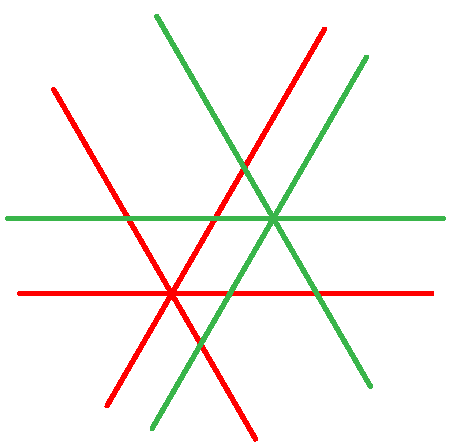
\includegraphics[scale=.4]{multiBraidArrangement2}
		&
		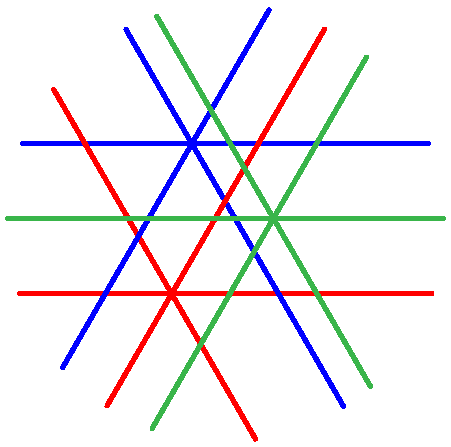
\includegraphics[scale=.4]{multiBraidArrangement3}
		&
		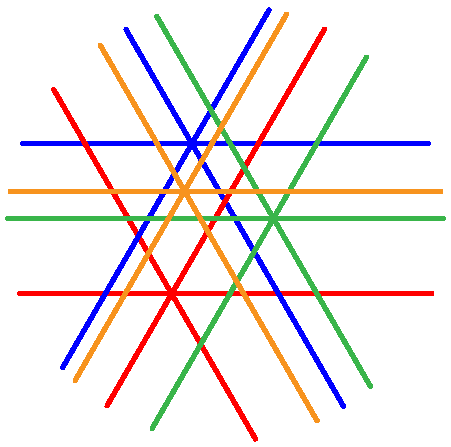
\includegraphics[scale=.4]{multiBraidArrangement4}
		\\
		$\ell = 1$ & $\ell = 2$ & $\ell = 3$ & $\ell = 4$
	\end{tabular}
	}
	\caption{The $(\ell,3)$-braid arrangements for~$\ell \in [4]$.}
	\label{fig:multiBraidArrangements}
\end{figure}

%\begin{definition}
%\label{def:multiBraidArrangement}
%The \defn{$(\ell,n)$-braid arrangement}~$\multiBraidArrangement$ is the arrangement in~$\HH$ obtained as the union of $\ell$ generically translated copies of the braid arrangement~$\braidArrangement$ (that is, the $\b{a}$-braid arrangement for some generic matrix~$\b{a} \in M_{\ell,n-1}(\R)$).
%\end{definition}
%
%This definition is slightly misleading, as the $(\ell,n)$-braid arrangement~$\multiBraidArrangement$ a priori depends on the (generic) translation vectors chosen for each copy.
%We will see that many combinatorial aspects of~$\multiBraidArrangement$, in particular its flat poset and thus its M\"obius, $f$- and $b$-polynomials, are in fact independent of the translation vectors as long as they are generic.
%However, the combinatorial description of the face poset of~$\multiBraidArrangement$ will depend on the translation vectors, so that we introduce the following more precise notation recording the translations.
%
%\begin{definition}
%A matrix~$\b{a} \eqdef (a_{i,j}) \in M_{\ell,n-1}(\R)$ is \defn{generic} if any linear dependence among its coefficients~$\sum_{i,j} \lambda_{i,j} \, a_{i,j} = 0$ splits into $\ell$ linear dependences~$\sum_j \lambda_{i,j} \, a_{i,j} = 0$ for~$i \in [\ell]$.
%\end{definition}
%
%\begin{definition}
%\label{def:multiBraidArrangementPrecise}
%For any integers~$\ell,n \geq 1$, and any matrix~$\b{a} \eqdef (a_{i,j}) \in M_{\ell,n-1}(\R)$, the \defn{$\b{a}$-braid arrangement}~$\multiBraidArrangement(\b{a})$ is the arrangement of hyperplanes~$\set{\b{x} \in \HH}{x_s - x_t = A_{i,s,t}}$ for all~${1 \le s < t \le n}$ and~$i \in [\ell]$, where $A_{i,s,t} \eqdef \smash{\sum_{s \le j < t} a_{i,j}}$.
%\end{definition}

\begin{definition}
\label{def:multiBraidArrangementPrecise}
For any integers~$\ell,n \geq 1$, and any matrix~$\b{a} \eqdef (a_{i,j}) \in M_{\ell,n-1}(\R)$, the \defn{$\b{a}$-braid arrangement}~$\multiBraidArrangement(\b{a})$ is the arrangement of hyperplanes~$\set{\b{x} \in \HH}{x_s - x_t = A_{i,s,t}}$ for all~${1 \le s < t \le n}$ and~$i \in [\ell]$, where $A_{i,s,t} \eqdef \smash{\sum_{s \le j < t} a_{i,j}}$.
\end{definition}

In other words, the $\b{a}$-braid arrangement~$\multiBraidArrangement(\b{a})$ is the union of~$\ell$ copies of the braid arrangement~$\braidArrangement$ translated according to the matrix~$\b{a}$.
Of course, the $\b{a}$-braid arrangement~$\multiBraidArrangement(\b{a})$ highly depends on~$\b{a}$.
In this paper, we are interested in the case where~$\b{a}$ is generic in the following sense.

\begin{definition}
A matrix~$\b{a} \eqdef (a_{i,j}) \in M_{\ell,n-1}(\R)$ is \defn{generic} if for any~$i_1, \dots, i_k \in [\ell]$ and distinct $r_1, \dots, r_k \in [n]$, the equality~$\sum_{j \in [k]} A_{i_j, r_{j-1}, r_j} = 0$ implies~$i_1 = \dots = i_k$ (with the notation~$A_{i,s,t} \eqdef \smash{\sum_{s \le j < t} a_{i,j}}$ and the convention~$r_0 = r_k$).
\end{definition}

We will see that many combinatorial aspects of~$\multiBraidArrangement(\b{a})$, in particular its flat poset and thus its M\"obius, $f$- and $b$-polynomials, are in fact independent of the matrix~$\b{a}$ as long as it is generic.
We therefore consider the following definition.

\begin{definition}
\label{def:multiBraidArrangement}
The \defn{$(\ell,n)$-braid arrangement}~$\multiBraidArrangement$ is the arrangement in~$\HH$ obtained as the union of $\ell$ generically translated copies of the braid arrangement~$\braidArrangement$ (that is, any $\b{a}$-braid arrangement for some generic matrix~$\b{a} \in M_{\ell,n-1}(\R)$).
\end{definition}

%\begin{remark}
%\label{rem:multiBraidArrangement}
%In practice, consider the hyperplanes~$\set{\b{x} \in \HH}{x_s - x_t = A_{i,s,t}}$ for all~$1 \le s < t \le n$ and~$i \in [\ell]$, where $A_{i,s,t} \eqdef \smash{\sum_{s \le j < t} a_{i,j}}$ for an arbitrary generic matrix~$(a_{i,j}) \in M_{\ell,n-1}(\R)$.
%\end{remark}

The objective of \cref{part:multiBraidArrangements} is to explore the combinatorics of these multiple braid arrangements.
We have split our presentation into two sections:
\begin{itemize}
\item In \cref{sec:flatPoset}, we describe the flat poset~$\flatPoset[\multiBraidArrangement]$ of the $(\ell,n)$-braid arrangement~$\multiBraidArrangement$ in terms of $(\ell,n)$-partition forests (\cref{subsec:partitionForests}) and labeled $(\ell,n)$-rainbow forests (\cref{subsec:rainbowForests}), which enables us to derive its M\"obius, $f$- and $b$- polynomials (\cref{subsec:MobiusPolynomialMultiBraidArrangement}), from which we extract interesting formulas for the number of vertices (\cref{subsec:verticesMultiBraidArrangement}) and regions (\cref{subsec:regionsMultiBraidArrangement}). Note that all these results are independent of the translation matrix.
\item In \cref{sec:facePoset}, we describe the face poset~$\facePoset[\multiBraidArrangement(\b{a})]$ of the $\b{a}$-braid  arrangement~$\multiBraidArrangement(\b{a})$ in terms of ordered $(\ell,n)$-partition forests (\cref{subsec:orderedPartitionForests}). In contrast to the flat poset, this description of the face poset depends on the translation matrix~$\b{a}$. For a given choice of~$\b{a}$, we describe in particular the ordered $(\ell,n)$-partitions forests with a given underlying (unordered) $(\ell,n)$-partition forest (\cref{subsec:PFtoOPF}). We then give a criterion to decide whether a given ordered $(\ell,n)$-partition forest corresponds to a face of~$\multiBraidArrangement(\b{a})$ (\cref{subsec:criterionOPF}).
\end{itemize}

\begin{remark}
Note that each hyperplane of the $(\ell,n)$-braid arrangement~$\multiBraidArrangement$ is orthogonal to a root~$\b{e}_i-\b{e}_j$ of the type~$A$ root system.
Many such arrangements have been studied previously, for instance, the \defn{Shi arrangement}~\cite{Shi1, Shi2}, the \defn{Catalan arrangement}~\cite[Sect.~7]{PostnikovStanley}, the \defn{Linial arrangement}~\cite[Sect.~8]{PostnikovStanley}, the \defn{generic arrangement} of~\cite[Sect.~5]{PostnikovStanley}, or the \defn{discriminantal arrangements} of~\cite{ManinSchechtman,BayerBrandt}.
We refer to the work of A.~Postnikov and R.~Stanley~\cite{PostnikovStanley} and of O.~Bernardi~\cite{Bernardi} for much more references.
However, in all these examples, either the copies of the braid arrangement are perturbed, or they are translated non-generically.
We have not been able to find the $(\ell,n)$-braid arrangement~$\multiBraidArrangement$ properly treated in the literature.
\end{remark}

\begin{remark}
Part of our discussion on the $(\ell,n)$-braid arrangement~$\multiBraidArrangement$ could actually be developed for a hyperplane arrangement~$\arrangement^\ell$ obtained as the union of~$\ell$ generically translated copies of an arbitrary linear hyperplane arrangement~$\arrangement$.
Similarly to \cref{prop:flatPosetMultiBraidArrangement}, the flat poset~$\flatPoset[\arrangement^\ell]$ is isomorphic to the lower set of the $\ell$\ordinal{} Cartesian power of the flat poset~$\flatPoset$ induced by the $\ell$-tuples whose meet in the flat poset~$\flatPoset$ is the bottom element~$\b{0}$ (these are sometimes called strong antichains) and which are minimal for this property.
Similar to \cref{thm:MobiusPolynomialMultiBraidArrangement}, this yields a general formula for the M\"obius polynomial of~$\arrangement^\ell$ in terms of the M\"obius function of the flat poset~$\flatPoset$.
Here, we additionally benefit from the nice properties of the M\"obius polynomial of the braid arrangement~$\braidArrangement$ to obtain appealing formulas for the vertices, regions and bounded regions of the $(\ell,n)$-braid arrangement~$\multiBraidArrangement$ (see \cref{thm:verticesMultiBraidArrangement,thm:verticesRefinedMultiBraidArrangement,thm:characteristicPolynomialMultiBraidArrangement,thm:regionsMultiBraidArrangement}).
We have therefore decided to restrict our attention to the $(\ell,n)$-braid arrangement~$\multiBraidArrangement$.
\end{remark}

%%%%%%%%%%%%%%%%%%%%%%%%%%%%%%%%%%%%%%

\section{Flat poset and enumeration of~$\multiBraidArrangement$}
\label{sec:flatPoset}

In this section, we describe the flat poset of the $(\ell,n)$-braid arrangement~$\multiBraidArrangement$ in terms of \mbox{$(\ell,n)$-partition} forests and derive explicit formulas for its $f$-vector.
Remarkably, the flat poset (and thus the M\"obius, $f$- and $b$- polynomials) of~$\multiBraidArrangement$ is independent of the translation vectors as long as they are generic.

%%%%%%%%%%%%%%%

\subsection{Partition forests}
\label{subsec:partitionForests}

We first introduce the main characters of this section, which will describe the combinatorics of the flat poset of the $(\ell,n)$-braid arrangement~$\multiBraidArrangement$ of \cref{def:multiBraidArrangement}.

\begin{definition}
\label{def:intersectionHypergraph}
The \defn{intersection hypergraph} of a $\ell$-tuple~$\b{F} \eqdef (F_1, \dots, F_\ell)$ of set partitions of~$[n]$ is the $\ell$-regular $\ell$-partite hypergraph on all parts of all the partitions~$F_i$ for~${i \in [\ell]}$, with a hyperedge connecting the parts containing~$j$  for each~$j \in [n]$.
\end{definition}

\begin{definition}
\label{def:partitionForests}
An \defn{$(\ell,n)$-partition forest} (\resp \defn{$(\ell,n)$-partition tree}) is a $\ell$-tuple~$\b{F} \eqdef (F_1, \dots, F_\ell)$ of set partitions of~$[n]$ whose intersection hypergraph is a hyperforest (\resp hypertree).
See \cref{fig:forests}.
The \defn{dimension} of~$\b{F}$ is~$\smash{{\dim(\b{F}) \eqdef n - 1 - \ell n + \sum_{i \in [\ell]} \card{F_i}}}$.
The \defn{$(\ell,n)$-partition forest poset} is the poset~$\forestPoset$ on $(\ell,n)$-partition forests ordered by componentwise refinement.
%
\begin{figure}[b]
	\centerline{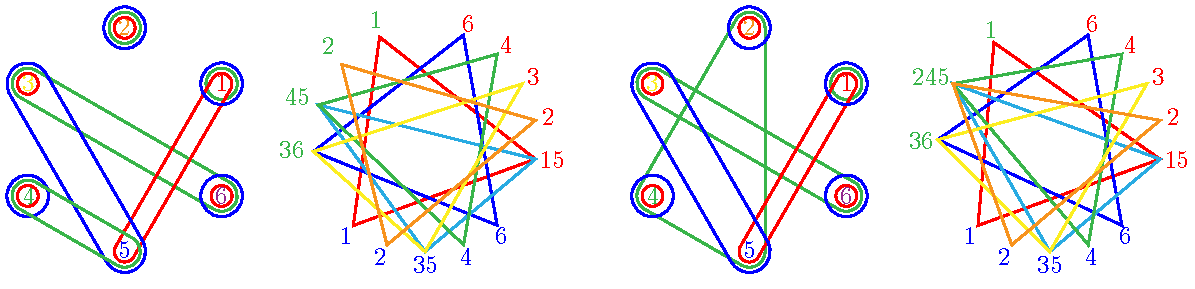
\includegraphics[scale=.9]{forests}}
	\caption{Some $(3,6)$-partition forests (top) with their intersection hypergraphs (middle) and the corresponding labeled $(3,6)$-rainbow forests (bottom). The last two are trees. The order of the colors in the bottom pictures is red, green, blue.}
	\label{fig:forests}
\end{figure}
\end{definition}

In other words, $\forestPoset$ is the lower set of the $\ell$\ordinal{} Cartesian power of the partition poset~$\partitionPoset$ induced by $(\ell,n)$-partition forests.
Note that the maximal elements of~$\forestPoset$ are the $(\ell, n)$-partition trees.

The following statement is illustrated in \cref{fig:intersectionPosetMultiBraidArrangement32}.
%
\begin{figure}
	\centerline{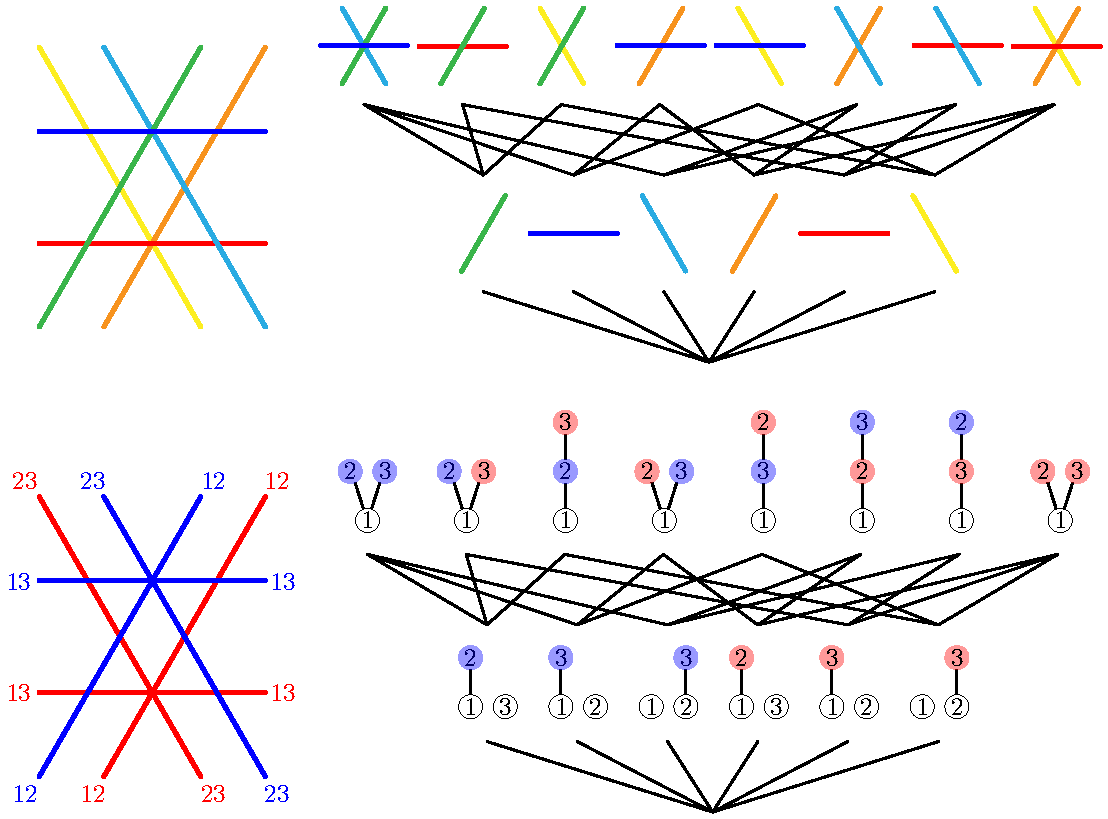
\includegraphics[scale=.9]{figures/intersectionPosetMultiBraidArrangement32Full}}
	\caption{The $(2,3)$-braid arrangement $\multiBraidArrangement[3][2]$ (left), and its flat poset (right), where flats are represented as intersections of hyperplanes (top), as $(2,3)$-partitions forests (middle), and as labeled $(2,3)$-rainbow forests (bottom).}
	\label{fig:intersectionPosetMultiBraidArrangement32}
\end{figure}

\begin{proposition}
\label{prop:flatPosetMultiBraidArrangement}
The flat poset~$\flatPoset[\multiBraidArrangement]$ of the $(\ell,n)$-braid arrangement~$\multiBraidArrangement$ is isomorphic to the $(\ell,n)$-partition forest poset.
\end{proposition}

\begin{proof}
Consider that~$\multiBraidArrangement$ is the $\b{a}$-braid arrangement~$\multiBraidArrangement(\b{a})$ for some generic matrix~$\b{a}$.
%Consider the hyperplanes~$\set{\b{x} \in \HH}{x_s - x_t = A_{i,s,t}}$ described in \cref{def:multiBraidArrangementPrecise}.
In view of our discussion in \cref{subsec:braidArrangement}, observe that, for each~${i \in [\ell]}$, each set partition~$\pi$ of~$[n]$ corresponds to a $(\card{\pi})$-dimensional flat
\[
\Psi_i(\pi) \eqdef \set{\b{x} \in \HH}{x_s - x_t = A_{i,s,t} \text{ for all $s,t$ in the same part of $\pi$} }
\]
of the $i$\ordinal{} copy of the braid arrangement~$\braidArrangement$.
The flats of the $(\ell,n)$-braid arrangement~$\multiBraidArrangement$ are thus all of the form
\[
\Psi(\b{F}) \eqdef \bigcap_{i \in [\ell]} \Psi_i(F_i)
\]
for certain $\ell$-tuples~$\b{F} \eqdef (F_1, \dots, F_\ell)$ of set partitions of~$[n]$.
Since the matrix~$\b{a}$ is generic, $\Psi(\b{F})$ is non-empty if and only if the intersection hypergraph of~$\b{F}$ is acyclic.
Moreover, $\Psi(\b{F})$ is included in~$\Psi(\b{G})$ if and only if~$\b{F}$ refines~$\b{G}$ componentwise.
Hence, the flat poset of~$\multiBraidArrangement$ is isomorphic to the $(\ell,n)$-partition forest poset.
Finally, notice that the codimension of the flat~$\Psi(\b{F})$ is the sum of the codimensions of the flats~$\Psi_i(F_i)$ for~$i \in [\ell]$, so that~$\dim(\b{F}) \eqdef n - 1 - \ell n + \sum_{i \in [\ell]} \card{F_i} $ is indeed the dimension of the flat~$\Psi(\b{F})$.
\end{proof}

%%%%%%%%%%%%%%%

\subsection{M\"obius polynomial}
\label{subsec:MobiusPolynomialMultiBraidArrangement}

We now derive from \cref{def:MobiusPolynomial,prop:flatPosetMultiBraidArrangement} the M\"obius polynomial of the $(\ell,n)$-braid arrangement~$\multiBraidArrangement$.

\begin{theorem}
\label{thm:MobiusPolynomialMultiBraidArrangement}
The M\"obius polynomial of the $(\ell,n)$-braid arrangement~$\multiBraidArrangement$ is given by
\[
\mobPol[\multiBraidArrangement] = x^{n-1-\ell n} y^{n-1-\ell n} \sum_{\b{F} \le \b{G}} \prod_{i \in [\ell]} x^{\card{F_i}} y^{\card{G_i}} \prod_{p \in G_i} (-1)^{\card{F_i[p]}-1} (\card{F_i[p]}-1)! \; ,
\]
where~$\b{F} \le \b{G}$ ranges over all intervals of the $(\ell,n)$-partition forest poset~$\forestPoset$, and~$F_i[p]$ denotes the restriction of the partition~$F_i$ to the part~$p$ of~$G_i$.
\end{theorem}

\begin{proof}
Observe that for~$\b{F} \eqdef (F_1, \dots, F_\ell)$ and~$\b{G} \eqdef (G_1, \dots, G_\ell)$ in~$\forestPoset$, we have
\[
[\b{F}, \b{G}] = \prod_{i \in [\ell]} [F_i, G_i] \simeq \prod_{i \in [\ell]} \prod_{p \in G_i} \partitionPoset[{\card{F_i[p]}}].
\]
Recall that the M\"obius function is multiplicative:
\(
\mu_{P \times Q} \big( (p,q), (p’,q’) \big) = \mu_P(p,p’) \cdot \mu_Q(q,q’),
\)
for all~$p, p' \in P$ and~$q, q' \in Q$.
Hence, we obtain that
\[
\mu_{\forestPoset}(\b{F}, \b{G}) = \prod_{i \in [\ell]} \prod_{p \in G_i} (-1)^{\card{F_i[p]}-1} (\card{F_i[p]}-1)! .
\]
Hence, we derive from \cref{def:MobiusPolynomial,prop:flatPosetMultiBraidArrangement} that
\begin{align*}
\mobPol[\multiBraidArrangement] 
& = \sum_{\b{F} \le \b{G}} \mu_{\forestPoset}(\b{F}, \b{G}) \, x^{\dim(\b{F})} \, y^{\dim(\b{G})} \\
& = x^{n-1-\ell n} y^{n-1-\ell n} \sum_{\b{F} \le \b{G}} \prod_{i \in [\ell]} x^{\card{F_i}} y^{\card{G_i}} \prod_{p \in G_i} (-1)^{\card{F_i[p]}-1} (\card{F_i[p]}-1)! .
\qedhere
\end{align*}
\end{proof}

By using the polynomial
\[
\weirdPol[n] \eqdef \mobPol[\braidArrangement][x][0] = \sum_{k \in [n]} (-1)^{k-1} \, (k-1)! \, S(n,k) \, x^{k-1}
\]
introduced at the end of \cref{subsec:braidArrangement}, the M\"obius polynomial~$\mobPol[\multiBraidArrangement]$ can also be expressed as follows.

\pagebreak
\begin{proposition} 
\label{prop:alternativeFormulaMobiusPolynomialMultiBraidArrangement}
The M\"obius polynomial of the $(\ell,n)$-braid arrangement~$\multiBraidArrangement$ is given by
\[
\mobPol[\multiBraidArrangement] = x^{(n-1)(1-\ell)} \sum_{G \in \forestPoset} y^{n-1-\ell n+\sum_{i \in [\ell]} \card{G_i}}  \prod_{i \in [\ell]} \weirdPol[\card{G_i}].
\]
\end{proposition}

\begin{proof}
As already mentioned, the $(\ell,n)$-partition forest poset~$\forestPoset$ is a lower set of the $\ell$\ordinal{} Cartesian power of the partition poset~$\partitionPoset$.
In other words, given a $(\ell,n)$-partition forest $\b{G} \eqdef (G_1, \dots, G_\ell)$, any $\ell$-tuple~$\b{F} \eqdef (F_1, \dots, F_\ell)$ of partitions satisfying~$F_i \le_{\partitionPoset[n]} G_i$ for all~$i \in [\ell]$ is a $(\ell,n)$-partition forest.
Hence, we obtain from \cref{def:MobiusPolynomial,prop:flatPosetMultiBraidArrangement} that
\begin{align*}
\mobPol[\multiBraidArrangement]
& = \sum_{G \in \forestPoset} y^{n-\ell n - 1 + \sum_{i \in [\ell]} \card{G_i}} \prod_{i \in [\ell]} \sum_{F_i \leq_{\partitionPoset[n]} G_i } \mu_{\partitionPoset[n]}(F_i,G_i) \, x^{n-\ell n - 1 + \sum_{i \in [\ell]} \card{F_i}}, \\
& = \sum_{G \in \forestPoset} y^{n-\ell n - 1 + \sum_{i \in [\ell]} \card{G_i}} x^{(n-1)(1-\ell)} \prod_{i \in [\ell]} \sum_{\pi_i \in \partitionPoset[\card{G_i}]}  \mu_{\partitionPoset[\card{G_i}]}(\pi_i,\hat{1}) \, x^{\card{\pi_i}-1}, 
\end{align*}
where $\hat{1}$ denotes the maximal element in $\partitionPoset[\card{G_i}]$ and $\pi_i$ is obtained from $F_i$ by merging elements in the same part of $G_i$.
The result follows since~$\weirdPol[\card{G_i}] = \sum_{\pi_i \in \partitionPoset[\card{G_i}]}  \mu_{\partitionPoset[\card{G_i}]}(\pi_i,\hat{1}) \, x^{\card{\pi_i}-1}$.
%Hence, we obtain
%\[
%\mobPol[\multiBraidArrangement] = \sum_{G \in \forestPoset} y^{n-\ell n - 1 + \sum_{i \in [\ell]} \card{G_i}} x^{(n-1)(1-\ell)} \prod_{i \in [\ell]} \weirdPol[\card{G_i}].
%\qedhere
%\]
\end{proof}

From \cref{thm:Zaslavsky,thm:MobiusPolynomialMultiBraidArrangement}, we thus obtain the face numbers and bounded face numbers of~$\multiBraidArrangement$, whose first few values are gathered in \cref{table:fvectorMultiBraidArrangements}.

%\begin{table}
%\centerline{
%	\begin{tabular}{c@{\hspace{.7cm}}c}
%		\begin{tabular}[t]{c|cccc|c}
%			$n \backslash k$ & $0$ & $1$ & $2$ & $3$ & $\Sigma$ \\
%			\hline
%			$1$ & $1$ &&&& $1$ \\
%			$2$ & $2$ & $1$ &&& $3$ \\
%			$3$ & $6$ & $6$ & $1$ && $13$ \\
%			$4$ & $24$ & $36$ & $14$ & $1$ & $75$
%		\end{tabular}
%		&
%		\begin{tabular}[t]{c|cccc|c}
%			$n \backslash k$ & $0$ & $1$ & $2$ & $3$ & $\Sigma$ \\
%			\hline
%			$1$ & $1$ &&&& $1$ \\
%			$2$ & $3$ & $2$ &&& $5$ \\
%			$3$ & $17$ & $24$ & $8$ && $49$ \\
%			$4$ & $149$ & $324$ & $226$ & $50$ & $749$
%		\end{tabular}
%		\\[2cm]
%		\begin{tabular}[t]{c|cccc|c}
%			$n \backslash k$ & $0$ & $1$ & $2$ & $3$ & $\Sigma$ \\
%			\hline
%			$1$ & $1$ &&&& $1$ \\
%			$2$ & $0$ & $1$ &&& $1$ \\
%			$3$ & $0$ & $0$ & $1$ && $1$ \\
%			$4$ & $0$ & $0$ & $0$ & $1$ & $1$
%		\end{tabular}
%		&
%		\begin{tabular}[t]{c|cccc|c}
%			$n \backslash k$ & $0$ & $1$ & $2$ & $3$ & $\Sigma$ \\
%			\hline
%			$1$ & $1$ &&&& $1$ \\
%			$2$ & $1$ & $2$ &&& $3$ \\
%			$3$ & $5$ & $12$ & $8$ && $25$ \\
%			$4$ & $43$ & $132$ & $138$ & $50$ & $363$
%		\end{tabular}
%		\\[2cm]
%		$\ell = 1$ & $\ell = 2$
%		\\[.8cm]
%		\begin{tabular}[t]{c|cccc|c}
%			$n \backslash k$ & $0$ & $1$ & $2$ & $3$ & $\Sigma$ \\
%			\hline
%			$1$ & $1$ &&&& $1$ \\
%			$2$ & $4$ & $3$ &&& $7$ \\
%			$3$ & $34$ & $54$ & $21$ && $109$ \\
%			$4$ & $472$ & $1152$ & $924$ & $243$ & $2791$
%		\end{tabular}
%		&
%		\begin{tabular}[t]{c|cccc|c}
%			$n \backslash k$ & $0$ & $1$ & $2$ & $3$ & $\Sigma$ \\
%			\hline
%			$1$ & $1$ &&&& $1$ \\
%			$2$ & $5$ & $4$ &&& $9$ \\
%			$3$ & $57$ & $96$ & $40$ && $193$ \\
%			$4$ & $1089$ & $2808$ & $2396$ & $676$ & $6969$
%		\end{tabular}
%		\\[2cm]
%		\begin{tabular}[t]{c|cccc|c}
%			$n \backslash k$ & $0$ & $1$ & $2$ & $3$ & $\Sigma$ \\
%			\hline
%			$1$ & $1$ &&&& $1$ \\
%			$2$ & $2$ & $3$ &&& $5$ \\
%			$3$ & $16$ & $36$ & $21$ && $73$ \\
%			$4$ & $224$ & $684$ & $702$ & $243$ & $1853$
%		\end{tabular}
%		&
%		\begin{tabular}[t]{c|cccc|c}
%			$n \backslash k$ & $0$ & $1$ & $2$ & $3$ & $\Sigma$ \\
%			\hline
%			$1$ & $1$ &&&& $1$ \\
%			$2$ & $3$ & $4$ &&& $7$ \\
%			$3$ & $33$ & $72$ & $40$ && $145$ \\
%			$4$ & $639$ & $1944$ & $1980$ & $676$ & $5239$
%		\end{tabular}
%		\\[2cm]
%		$\ell = 3$ & $\ell = 4$
%	\end{tabular}
%	}
%	\vspace{.3cm}
%	\caption{The face numbers (top) and the bounded face numbers (bottom) of the $(\ell,n)$-braid arrangements for~$\ell, n \in [4]$.}
%	\label{table:fvectorMultiBraidArrangements}
%\end{table}

\begin{table}[t]
	\centerline{\scalebox{.8}{
		\begin{tabular}{c@{\hspace{.7cm}}c@{\hspace{.7cm}}c@{\hspace{.7cm}}c}
			$\ell = 1$ & $\ell = 2$ & $\ell = 3$ & $\ell = 4$
			\\[.2cm]
			\begin{tabular}[t]{c|cccc|c}
				$n \backslash k$ & $0$ & $1$ & $2$ & $3$ & $\Sigma$ \\
				\hline
				$1$ & $1$ &&&& $1$ \\
				$2$ & $2$ & $1$ &&& $3$ \\
				$3$ & $6$ & $6$ & $1$ && $13$ \\
				$4$ & $24$ & $36$ & $14$ & $1$ & $75$
			\end{tabular}
			&
			\begin{tabular}[t]{c|cccc|c}
				$n \backslash k$ & $0$ & $1$ & $2$ & $3$ & $\Sigma$ \\
				\hline
				$1$ & $1$ &&&& $1$ \\
				$2$ & $3$ & $2$ &&& $5$ \\
				$3$ & $17$ & $24$ & $8$ && $49$ \\
				$4$ & $149$ & $324$ & $226$ & $50$ & $749$
			\end{tabular}
			&
			\begin{tabular}[t]{c|cccc|c}
				$n \backslash k$ & $0$ & $1$ & $2$ & $3$ & $\Sigma$ \\
				\hline
				$1$ & $1$ &&&& $1$ \\
				$2$ & $4$ & $3$ &&& $7$ \\
				$3$ & $34$ & $54$ & $21$ && $109$ \\
				$4$ & $472$ & $1152$ & $924$ & $243$ & $2791$
			\end{tabular}
			&
			\begin{tabular}[t]{c|cccc|c}
				$n \backslash k$ & $0$ & $1$ & $2$ & $3$ & $\Sigma$ \\
				\hline
				$1$ & $1$ &&&& $1$ \\
				$2$ & $5$ & $4$ &&& $9$ \\
				$3$ & $57$ & $96$ & $40$ && $193$ \\
				$4$ & $1089$ & $2808$ & $2396$ & $676$ & $6969$
			\end{tabular}
			\\[2.3cm]
			\begin{tabular}[t]{c|cccc|c}
				$n \backslash k$ & $0$ & $1$ & $2$ & $3$ & $\Sigma$ \\
				\hline
				$1$ & $1$ &&&& $1$ \\
				$2$ & $0$ & $1$ &&& $1$ \\
				$3$ & $0$ & $0$ & $1$ && $1$ \\
				$4$ & $0$ & $0$ & $0$ & $1$ & $1$
			\end{tabular}
			&
			\begin{tabular}[t]{c|cccc|c}
				$n \backslash k$ & $0$ & $1$ & $2$ & $3$ & $\Sigma$ \\
				\hline
				$1$ & $1$ &&&& $1$ \\
				$2$ & $1$ & $2$ &&& $3$ \\
				$3$ & $5$ & $12$ & $8$ && $25$ \\
				$4$ & $43$ & $132$ & $138$ & $50$ & $363$
			\end{tabular}
			&
			\begin{tabular}[t]{c|cccc|c}
				$n \backslash k$ & $0$ & $1$ & $2$ & $3$ & $\Sigma$ \\
				\hline
				$1$ & $1$ &&&& $1$ \\
				$2$ & $2$ & $3$ &&& $5$ \\
				$3$ & $16$ & $36$ & $21$ && $73$ \\
				$4$ & $224$ & $684$ & $702$ & $243$ & $1853$
			\end{tabular}
			&
			\begin{tabular}[t]{c|cccc|c}
				$n \backslash k$ & $0$ & $1$ & $2$ & $3$ & $\Sigma$ \\
				\hline
				$1$ & $1$ &&&& $1$ \\
				$2$ & $3$ & $4$ &&& $7$ \\
				$3$ & $33$ & $72$ & $40$ && $145$ \\
				$4$ & $639$ & $1944$ & $1980$ & $676$ & $5239$
			\end{tabular}
		\end{tabular}
	}}
%	\vspace{.3cm}
	\caption{The face numbers (top) and the bounded face numbers (bottom) of the $(\ell,n)$-braid arrangements for~$\ell, n \in [4]$.}
	\label{table:fvectorMultiBraidArrangements}
\end{table}

\begin{corollary}
\label{coro:fbvectorsMultiBraidArrangement}
The $f$- and $b$-polynomials of the $(\ell,n)$-braid arrangement~$\multiBraidArrangement$ are given by
\begin{align*}
\fPol[\multiBraidArrangement] & = x^{n-1-\ell n}\sum_{\b{F} \le \b{G}} \prod_{i \in [\ell]} x^{\card{F_i}} \prod_{p \in G_i} (\card{F_i[p]}-1)!\\
\text{and}\qquad
\bPol[\multiBraidArrangement] & = (-1)^\ell x^{n-1-\ell n} \sum_{\b{F} \le \b{G}} \prod_{i \in [\ell]} x^{\card{F_i}} \prod_{p \in G_i} -(\card{F_i[p]}-1)! ,
\end{align*}
where~$\b{F} \le \b{G}$ ranges over all intervals of the $(\ell,n)$-partition forest poset~$\forestPoset$, and~$F_i[p]$ denotes the restriction of the partition~$F_i$ to the part~$p$ of~$G_i$.
\end{corollary}

\begin{example}
For~$n = 1$, we have
\[
\mobPol[{\multiBraidArrangement[1][\ell]}] = \fPol[{\multiBraidArrangement[1][\ell]}] = \bPol[{\multiBraidArrangement[1][\ell]}] = 1.
\]
For~$n = 2$, we have
\[
\mobPol[{\multiBraidArrangement[2][\ell]}] = xy-\ell x+\ell,
\quad
\fPol[{\multiBraidArrangement[2][\ell]}] = (\ell+1)x+\ell
\quad\text{and}\quad
\bPol[{\multiBraidArrangement[2][\ell]}] = (\ell-1)x+\ell.
\]
The case~$n = 3$ is already more interesting.
Consider the set partitions~$P \eqdef \big\{ \{1\}, \{2\}, \{3\} \big\}$, $Q_i \eqdef \big\{ \{i\}, [3] \ssm \{i\} \big\}$ for~$i \in [3]$, and~$R \eqdef \big\{ [3] \big\}$.
Observe that the $(\ell,3)$-partition forests are all of the form
\begin{gather*}
\b{F} \eqdef P^\ell,
\quad
\b{G}_i^p \eqdef P^p Q_i P^{\ell-p-1}, % \text{ for } p \le \ell-1 \text{ and } i \in [3],
\quad
\b{H}_{i,j}^{p,q} \eqdef P^p Q_i P^{\ell-p-q-2} Q_j P^q \;\text{($i \ne j$)} % \text{ for } p + q \le \ell-2 \text{ and } i \ne j \in [3]
\quad\text{or}\quad
\b{K}^p \eqdef P^p R P^{\ell-p-1}. % \text{ for } p \le \ell-1.
\end{gather*}
(where we write a tuple of partitions of~$[3]$ as a word on~$\{P, Q_1, Q_2, Q_3, R\}$). %, and $p$ and $q$ are such that the total length is~$\ell$).
%\begin{gather*}
%\b{F} \eqdef (\underbrace{P, \dots, P}_\ell), \\
%\b{G}_i^p \eqdef (\underbrace{P, \dots, P}_p, Q_i, \underbrace{P, \dots, P}_{\ell-p-1}) \text{ for } p \le \ell-1 \text{ and } i \in [3],
%\\
%\b{H}_{i,j}^{p,q} \eqdef (\underbrace{P, \dots, P}_p, Q_i, \underbrace{P, \dots, P}_{\ell-p-q-2}, Q_j, \underbrace{P, \dots, P}_q) \text{ for } p + q \le \ell-2 \text{ and } i \ne j \in [3],
%\\
%\text{or}\quad
%\b{K}^p \eqdef (\underbrace{P, \dots, P}_p, R, \underbrace{P, \dots, P}_{\ell-p-1}) \text{ for } p \le \ell-1.
%\end{gather*}
Moreover, the cover relations in the $(\ell,3)$-partition forest poset are precisely the relations
\[
\b{F} \le \b{G}_i^p \hspace{-.4cm} \begin{array}{l} \rotatebox[origin=c]{45}{$\le$} \raisebox{.2cm}{$\b{H}_{i,j}^{p,q}$} \\[.1cm] \quad \le \b{K}^p \\[.1cm] \rotatebox[origin=c]{-45}{$\le$} \raisebox{-.2cm}{$\b{H}_{j,i}^{\ell-q-1, \ell-p-1}$} \end{array}
\]
for~$i \ne j$ and~$p, q$ such that~$p + q \le \ell-2$.
Hence, we have
\begin{align*}
\mobPol[{\multiBraidArrangement[3][\ell]}] & = x^2 y^2 - 3 \ell x^2 y + \ell (3 \ell - 1) x^2 + 3 \ell x y - 3 \ell (2 \ell - 1) x + \ell (3 \ell - 2) , \\
\fPol[{\multiBraidArrangement[3][\ell]}] & = (3 \ell^2 + 2 \ell + 1) x^2 + 6 \ell^2 x + \ell (3 \ell - 2), \\
\text{and}\qquad
\bPol[{\multiBraidArrangement[3][\ell]}] & = (3 \ell^2 - 4 \ell + 1) x^2 + 6 \ell (\ell - 1) x + \ell (3 \ell - 2).
\end{align*}
Observe that~$3 \ell^2 + 2 \ell + 1$ is~\OEIS{A056109}, that~$\ell (3 \ell - 2)$ is~\OEIS{A000567}, and that ${3 \ell^2 - 4 \ell + 1}$ is~\OEIS{A045944}.
%\vincenti{There is a weird connection between the first and the last. Namely, $3 \ell^2 - 4 \ell + 1 = 3 (\ell - 1)^2 + 2 (\ell - 1)$. Is there a bijective explanation on the arrangements?}
\end{example}

%%%%%%%%%%%%%%%

\subsection{Rainbow forests}
\label{subsec:rainbowForests}

In order to obtain more explicit formulas for the number of vertices and regions of the $(\ell,n)$-braid arrangement~$\multiBraidArrangement$ in \cref{subsec:verticesMultiBraidArrangement,subsec:regionsMultiBraidArrangement}, we now introduce another combinatorial model for $(\ell,n)$-partition forests which is more adapted to their enumeration.

\begin{definition}
\label{def:rainbowForest}
An \defn{$\ell$-rainbow coloring} of a rooted plane forest~$F$ is an assignment of colors of~$[\ell]$ to the non-root nodes of~$F$ such that
\begin{enumerate}[(i)]
\item there is no monochromatic edge,
\item the colors of siblings are increasing from left to right.
\end{enumerate}
We denote by~$\|F\|$ the number of nodes of~$F$ and by~$\card{F}$ the number of trees of the forest~$F$ (\ie its number of connected components).
An \defn{$(\ell,n)$-rainbow forest} (\resp \defn{tree}) is a \mbox{$\ell$-rainbow} colored forest (\resp tree) with $\|F\| = n$ nodes.
We denote by~$\rainbowForests$ (\resp $\rainbowTrees$) the set of $(\ell,n)$-rainbow forests (\resp trees), and set~$\rainbowForests[][\ell] \eqdef \bigsqcup_n \rainbowForests$ (\resp $\rainbowTrees[][\ell] \eqdef \bigsqcup_n \rainbowTrees$).
\end{definition}

For instance, we have listed the $14$ $(2,4)$-rainbow trees in \cref{fig:rainbowTrees}\,(top).
This figure actually illustrates the following statement.

\begin{lemma}
\label{lem:FussCatalan}
The $(\ell,m)$-rainbow trees are counted by the \defn{Fuss-Catalan number}
\[
\card{\rainbowTrees[m][\ell]} = F_{\ell,m} \eqdef \frac{1}{(\ell-1)m+1} \binom{\ell m}{m} \qquad \text{\OEIS{A062993}}.
\]
\end{lemma}

\begin{proof}
We can transform a $\ell$-rainbow tree~$R$ to an $\ell$-ary tree~$T$ as illustrated in \cref{fig:rainbowTrees}.
Namely, the parent of a node~$N$ in~$T$ is the previous sibling colored as~$N$ in~$R$ if it exists, and the parent of~$N$ in~$R$ otherwise.
This classical map is a bijection from $\ell$-rainbow trees to $\ell$-ary trees, which are counted by the Fuss-Catalan numbers~\cite{Klarner, HiltonPedersen}.
%
\begin{figure}
	\centerline{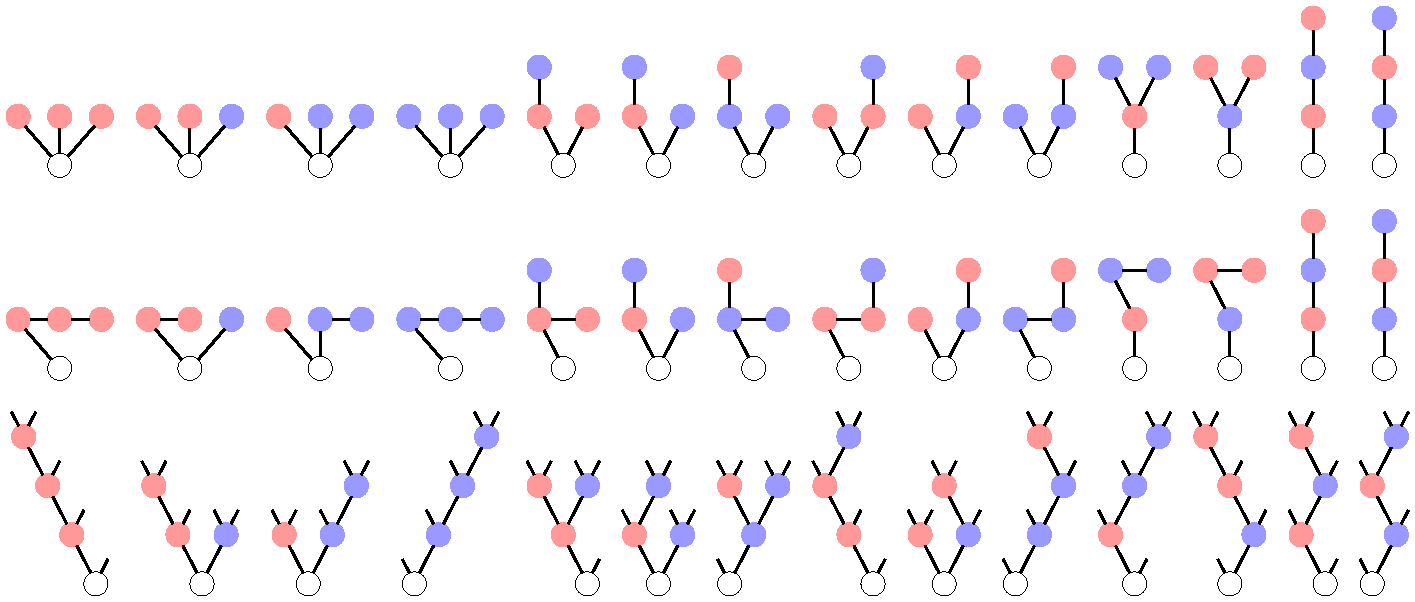
\includegraphics[scale=.7]{rainbowTrees}}
	\caption{The $14$ $(2,4)$-rainbow trees (top) and $14$ binary trees (bottom), and the simple bijection between them (middle). The order of the colors is red, blue.}
	\label{fig:rainbowTrees}
\end{figure}
\end{proof}

\begin{remark}
\label{rem:functionalEquationFussCatalan}
Recall that the corresponding generating function~$F_\ell(z) \eqdef \sum_{m \ge 0} F_{\ell,m} \, z^m$ satisfies the functional equation
\[
F_\ell(z) = 1 + z \, F_\ell(z)^\ell.
\]
\end{remark}

\begin{table}
	\centerline{\scalebox{.8}{
		\begin{tabular}[t]{c|ccccccccc}
			$m \backslash \ell$ & $1$ & $2$ & $3$ & $4$ & $5$ & $6$ & $7$ & $8$ & $9$ \\
			\hline
			$1$ & $1$ & $1$ & $1$ & $1$ & $1$ & $1$ & $1$ & $1$ & $1$ \\
			$2$ & $1$ & $2$ & $3$ & $4$ & $5$ & $6$ & $7$ & $8$ & $9$ \\
			$3$ & $1$ & $5$ & $12$ & $22$ & $35$ & $51$ & $70$ & $92$ & $117$ \\
			$4$ & $1$ & $14$ & $55$ & $140$ & $285$ & $506$ & $819$ & $1240$ & $1785$ \\
			$5$ & $1$ & $42$ & $273$ & $969$ & $2530$ & $5481$ & $10472$ & $18278$ & $29799$ \\
			$6$ & $1$ & $132$ & $1428$ & $7084$ & $23751$ & $62832$ & $141778$ & $285384$ & $527085$ \\
			$7$ & $1$ & $429$ & $7752$ & $53820$ & $231880$ & $749398$ & $1997688$ & $4638348$ & $9706503$ \\
			$8$ & $1$ & $1430$ & $43263$ & $420732$ & $2330445$ & $9203634$ & $28989675$ & $77652024$ & $184138713$ \\
			$9$ & $1$ & $4862$ & $246675$ & $3362260$ & $23950355$ & $115607310$ & $430321633$ & $1329890705$ & $3573805950$
		\end{tabular}
	}}
%	\vspace{.3cm}
	\caption{The Fuss-Catalan numbers~$F_{\ell,m} = \frac{1}{(\ell-1)m+1} \binom{\ell m}{m}$ for~$\ell,m \in [9]$. See \OEIS{A062993}.}
\end{table}

\begin{definition}
For a $(\ell,n)$-rainbow forest~$F$, we define
\[
\omega(F) \eqdef \prod_{i \in [\ell]} \prod_{N \in F} \card{C_i(N)}! ,
\]
where~$N$ ranges over all nodes of~$F$ and~$C_i(N)$ denotes the children of~$N$ colored by~$i$.
\end{definition}

\begin{definition}
\label{def:labelingRainbowForest}
A \defn{labeling} of a $(\ell,n)$-rainbow forest~$F$ is a bijective map from the nodes of~$F$ to~$[n]$ such that
\begin{enumerate}[(i)]
\item the label of each root is minimal in its tree,
\item the labels of siblings with the same color are increasing from left to right.
\end{enumerate}
\end{definition}

\begin{lemma}
\label{lem:labelingRainbowForest}
The number~$\lambda(F)$ of labelings of a $(\ell,n)$-rainbow forest~$F$ is given by
\[
\lambda(F) = \frac{n!}{\omega(F) \prod\limits_{T \in F} \|T\|} .
\]
\end{lemma}

\begin{proof}
Out of all~$n!$ bijective maps from the nodes of~$F$ to~$[n]$, only~$1/\prod_{T \in F} \|T\|$ satisfy Condition~(i) of \cref{def:labelingRainbowForest}, and only $1/\prod_{i \in [\ell]} \prod_{N \in F} \card{C_i(N)}! = 1/\omega(F)$ satisfy Condition~(ii) of \cref{def:labelingRainbowForest}.
\end{proof}

The following statement is illustrated in \cref{fig:forests}.

\begin{proposition}
\label{prop:bijectionForests}
There is a bijection from $(\ell,n)$-partition forests to labeled $(\ell,n)$-rainbow forests, such that if the partition forest~$\b{F}$ is sent to the labeled rainbow forest~$F$, then
\[
\dim(\b{F}) = \card{F}-1
\qquad\text{and}\qquad
\mu_{\forestPoset}(\HH, \b{F}) = (-1)^{n-\card{F}} \, \omega(F).
\]
\end{proposition}

\begin{proof}
From a labeled $(\ell,n)$-rainbow forest~$F$, we construct a $(\ell,n)$-partition forest~$\b{F} \eqdef (F_1, \dots, F_\ell)$ whose $i$\ordinal{} partition~$F_i$ has a part~$\{N\} \cup C_i(N)$ for each node~$N$ of~$F$ not colored~$i$.
Condition~(i) of \cref{def:rainbowForest} ensures that each $F_i$ is indeed a partition.

Conversely, start from a $(\ell,n)$-partition forest~$\b{F} \eqdef (F_1, \dots, F_i)$.
Consider the colored clique graph~$K_{\b{F}}$ on~$[n]$ obtained by replacing each part in~$F_i$ by a clique of edges colored by~$i$.
For each~$1 < j \le n$, there is a unique shortest path in~$K_{\b{F}}$ from the vertex~$j$ to the smallest vertex in the connected component of~$j$.
Define the parent~$p$ of~$j$ to be the next vertex along this path, and color the node~$j$ by the color of the edge between~$j$ and~$p$.
This defines a labeled $(\ell,n)$-rainbow forest~$F$.

Finally, observe that
\begin{gather*}
\dim(\b{F}) = n - 1 - \ell n + \sum_{i \in [\ell]} \card{F_i} = \card{F}-1, \qquad\text{and} \\
\mu_{\forestPoset}(\HH, \b{F}) = \prod\limits_{i \in [\ell]} \prod\limits_{p \in F_i} (-1)^{\card{p}-1} (\card{p}-1) = \prod\limits_{i \in [\ell]} \prod\limits_{N \in F} (-1)^{\card{C_i(N)}} \card{C_i(N)}! = (-1)^{n-\card{F}} \, \omega(F).
\qedhere
\end{gather*}
\end{proof}

We now transport via this bijection the partial order of the flat lattice on rainbow forests.
For a node~$a$ of a forest~$F$, we denote by $\operatorname{Root}(a)$ the root of the tree of~$F$ containing~$a$.
The following statement is illustrated in \cref{fig:CoverRelRF}, choosing $c$ to be green, $a$ to be $5$ and $b$ to be $7$.

\begin{figure}
	\centerline{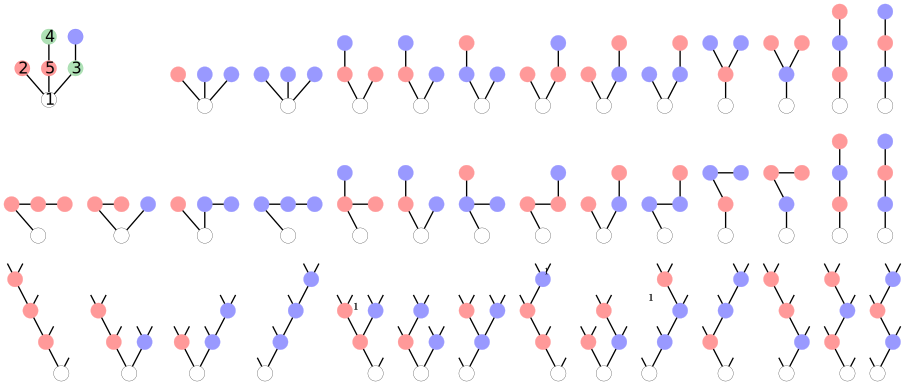
\includegraphics[scale=1]{CoverRelRFFig}}
	\vspace{-.3cm}
	\caption{A covering relation described in \cref{prop:CoverRelRF}, choosing $c$ to be green, $a$ to be $5$ and $b$ to be $7$.}
	\label{fig:CoverRelRF}
\end{figure}

\begin{proposition}
\label{prop:CoverRelRF}
In the flat poset~$\flatPoset[\multiBraidArrangement]$ labeled by rainbow forests using~\cref{prop:flatPosetMultiBraidArrangement,prop:bijectionForests}, a rainbow forest~$F$ is covered by a rainbow forest~$G$ if and only $G$ can be obtained from $F$ by:
\begin{enumerate}
\item choosing a color $c$, and two vertices $a$ and $b$ not colored with~$c$ and with~$\operatorname{Root}(a)<\operatorname{Root}(b)$,
\item shifting the colors along the path from~$\operatorname{Root}(b)$ to~$b$, so that each node along this path is now colored by the former color of its child and~$b$ is not colored anymore,
\item rerooting at~$b$ the tree containing~$b$ at~$b$, and coloring $b$ with~$c$,
\item adding an edge~$(a,b)$ and replacing the edge~$(b,e)$ by an edge~$(a,e)$ for each child $e$ of~$b$ colored with~$c$.
\end{enumerate}
\end{proposition}

\begin{proof}
Let us first remark that the graph obtained by these operations is indeed a rainbow forest.
First, we add an edge between two distinct connected components, so that the result is indeed acyclic.
Moreover, the condition on the color of $a$ and on the deletion of edges between $b$ and vertices of color $c$ ensures that we do not add an edge between two vertices of the same color.
Note that the parent of $b$ inherits the color of $b$ which is not $c$.

Let us recall that the cover relations in the flat poset~$\flatPoset[\multiBraidArrangement]$ are given in terms of $(\ell,n)$-partition forests by choosing a partition $\pi$ of the partition tuple (which corresponds directly to choosing a color), choosing two parts $\pi_a$ and $\pi_b$ in the partition $\pi$, and merging them, without creating a loop in the intersection hypergraph.

By choosing two vertices in different connected components of the rainbow forest, we are sure that the intersection hypergraph obtained by adding an edge is still acyclic.

The last point that has to be explained is the link between the condition on the color of~$a$ and~$b$ and merging two parts in the same partition.
If one of the two nodes, say $a$ for instance is of color~$c$, then it belongs to the same part of $\pi$ as its parent $z$.
The merging is the same if we choose~$z$ which is not colored $c$.
Moreover, as $b$ is in a different connected component, the corresponding two parts are distinct in $\pi$.
Finally, a part is just a corolla so the merging corresponds to building a corolla with $a$, $b$ and their children of color $c$.
\end{proof}

We finally recast \cref{prop:alternativeFormulaMobiusPolynomialMultiBraidArrangement} in terms of rainbow forests.

\begin{proposition} 
The M\"obius polynomial of the $(\ell,n)$-braid arrangement~$\multiBraidArrangement$ is given by
\[
\mobPol[\multiBraidArrangement] = x^{(n-1)(1-\ell)} \sum_{G \in \rainbowForests} y^{n-1+\card{E(G)}}  \prod_{i \in [\ell]} \weirdPol[n-\card{E(G,i)}].
\]
\end{proposition}

\begin{remark}
To further simplify this expression, we would need to count the number of rainbow forests with a prescribed number of colored edges.
However, this number does not admit a known multiplicative formula, up to our knowledge. When there is only one color, the corresponding sequence (counting non-colored forests on $n$ nodes and $k$ edges, rooted in the minimal label of each connected component) is \OEIS{A138464}.
\end{remark}

%%%%%%%%%%%%%%%

\subsection{Enumeration of vertices of $\multiBraidArrangement$}
\label{subsec:verticesMultiBraidArrangement}

We now use the labeled $(\ell,n)$-rainbow forests of \cref{subsec:rainbowForests} to derive more explicit formulas for the number of vertices of the $(\ell,n)$-braid arrangement~$\multiBraidArrangement$.
The first few values are gathered in \cref{table:verticesMultiBraidArrangement}.
 
\begin{table}
	\centerline{\scalebox{.8}{
		\begin{tabular}[t]{c|cccccccc}
			$n \backslash \ell$ & $1$ & $2$ & $3$ & $4$ & $5$ & $6$ & $7$ & $8$ \\ % & $9$ \\
			\hline
		$1$ & $1$ & $1$ & $1$ & $1$ & $1$ & $1$ & $1$ & $1$ \\ % & $1$ \\
		$2$ & $1$ & $2$ & $3$ & $4$ & $5$ & $6$ & $7$ & $8$ \\ % & $9$ \\
		$3$ & $1$ & $8$ & $21$ & $40$ & $65$ & $96$ & $133$ & $176$ \\ % & $225$ \\
		$4$ & $1$ & $50$ & $243$ & $676$ & $1445$ & $2646$ & $4375$ & $6728$ \\ % & $9801$ \\
		$5$ & $1$ & $432$ & $3993$ & $16384$ & $46305$ & $105456$ & $208537$ & $373248$ \\ % & $620289$ \\
		$6$ & $1$ & $4802$ & $85683$ & $521284$ & $1953125$ & $5541126$ & $13119127$ & $27350408$ \\ % & $51883209$ \\
		$7$ & $1$ & $65536$ & $2278125$ & $20614528$ & $102555745$ & $362797056$ & $1029059101$ & $2500000000$ \\ % & $5415228513$ \\
		$8$ & $1$ & $1062882$ & $72412707$ & $976562500$ & $6457339845$ & $28500625446$ & $96889010407$ & $274371577992$ % \\ & $678770015625$ \\
%		$9$ & $1$ & $20000000$ & $2681615217$ & $53971714048$ & $474659385665$ & $2614905943296$ & $10657046640625$ & $35184372088832$ & $99426586671873$
		\end{tabular}
	}}
%	\vspace{.3cm}
	\caption{The numbers $f_0(\multiBraidArrangement) = \ell \big( (\ell-1) n + 1 \big)^{n-2}$ of vertices of~$\multiBraidArrangement$ for~$\ell,n \in [8]$.}
	\label{table:verticesMultiBraidArrangement}
\end{table}

\begin{theorem}
\label{thm:verticesMultiBraidArrangement}
The number of vertices of the $(\ell,n)$-braid arrangement~$\multiBraidArrangement$ is
\[
f_0(\multiBraidArrangement) = \ell \big( (\ell-1) n + 1 \big)^{n-2}.
\]
\end{theorem}

\begin{proof}
By \cref{prop:flatPosetMultiBraidArrangement,prop:bijectionForests}, we just need to count the labeled $(\ell,n)$-rainbow trees.
A common reasoning for counting Cayley trees is the use of its Prüfer code defined by recursively pruning the smallest leaf while writing down the label of its parent.
This bijection can be adapted to colored Cayley trees by writing down the label of the parent colored by the color of the pruned leaf.
This leads to a bijection with certain colored words of length $n-1$.
Namely, there are two possibilities:
\begin{itemize}
\item either the pruned leaf is attached to the node~$1$ and it can have all $\ell$ colors,
\item or it is attached to one of the $n-1$ other nodes and it can only have $\ell-1$ colors.
\end{itemize}
Note that the last letter in the Prüfer code (obtained by removing the last edge) is necessarily the root $1$, with $\ell$ possible different colors.
Hence, there are 
\[
\big( \ell+(n-1)(\ell-1) \big)^{n-2} \ell = \ell \big( (\ell-1) n + 1 \big)^{n-2}
\]
such words.
Similar ideas were used in~\cite{Lewis}.
\end{proof}

We can refine the formula of \cref{thm:verticesMultiBraidArrangement} according to the dimension of the flats of the different copies intersected to obtain the vertices of the $(\ell,n)$-braid arrangement~$\multiBraidArrangement$.

\begin{theorem}
\label{thm:verticesRefinedMultiBraidArrangement}
For any~$k_1, \dots, k_\ell$ such that~$0 \le k_i \le n-1$ for~$i \in [\ell]$ and~${\sum_{i \in [\ell]} k_i = n-1}$, the number of vertices~$v$ of the $(\ell,n)$-braid arrangement~$\multiBraidArrangement$ such that the smallest flat of the $i$\ordinal{} copy of~$\braidArrangement$ containing~$v$ has dimension~$n-k_i-1$ is given by
\[
n^{\ell-1} \binom{n-1}{k_1, \dots, k_\ell} \prod_{i \in [\ell]} (n-k_i)^{k_i-1}.
\]
\end{theorem}

\begin{proof}
By \cref{prop:flatPosetMultiBraidArrangement,prop:bijectionForests}, we just need to count the labeled $(\ell,n)$-rainbow trees with~$k_i$ nodes colored by~$i$.
Forgetting the labels, the $(\ell,n)$-rainbow trees with~$k_i$ nodes colored by~$i$ are precisely the spanning trees of the complete multipartite graph~$K_{k_1, \dots, k_\ell, 1}$ (where the last~$1$ stands for the uncolored root).
Using a Pr\"ufer code similar to that of the proof of \cref{thm:verticesMultiBraidArrangement}, R.~Lewis proved in~\cite{Lewis} that the latter are counted by~${n^{\ell-1} \prod_{i \in [\ell]} (n-k_i)^{k_i-1}}$.
Finally, the possible labelings are counted by the multinomial coefficient~$\binom{n-1}{k_1, \dots, k_\ell}$.
\end{proof}

%%%%%%%%%%%%%%%

\subsection{Enumeration of regions and bounded regions of $\multiBraidArrangement$}
\label{subsec:regionsMultiBraidArrangement}

\enlargethispage{.2cm}
We finally use the labeled $(\ell,n)$-rainbow forests of \cref{subsec:rainbowForests} to derive more explicit formulas for the number of regions and bounded regions of the $(\ell,n)$-braid arrangement~$\multiBraidArrangement$.
The first few values are gathered in \cref{table:regionsMultiBraidArrangement,table:boundedRegionsMultiBraidArrangement}.
We first compute the characteristic polynomial of~$\multiBraidArrangement$.

\afterpage{
\begin{table}
	\centerline{\scalebox{.8}{
		\begin{tabular}[t]{c|cccccccc}
			$n \backslash \ell$ & $1$ & $2$ & $3$ & $4$ & $5$ & $6$ & $7$ & $8$ \\ % & $9$ \\
			\hline
			$1$ & $1$ & $1$ & $1$ & $1$ & $1$ & $1$ & $1$ & $1$ \\ % & $1$ \\
			$2$ & $2$ & $3$ & $4$ & $5$ & $6$ & $7$ & $8$ & $9$ \\ % & $10$ \\
			$3$ & $6$ & $17$ & $34$ & $57$ & $86$ & $121$ & $162$ & $209$ \\ % & $262$ \\
			$4$ & $24$ & $149$ & $472$ & $1089$ & $2096$ & $3589$ & $5664$ & $8417$ \\ % & $11944$ \\
			$5$ & $120$ & $1809$ & $9328$ & $29937$ & $73896$ & $154465$ & $287904$ & $493473$ \\ % & $793432$ \\
			$6$ & $720$ & $28399$ & $241888$ & $1085157$ & $3442816$ & $8795635$ & $19376064$ & $38323753$ \\ % & $69841072$ \\
			$7$ & $5040$ & $550297$ & $7806832$ & $49075065$ & $200320816$ & $625812385$ & $1629858672$ & $3720648337$ \\ % & $7686190000$ \\
			$8$ & $40320$ & $12732873$ & $302346112$ & $2666534049$ & $14010892416$ & $53536186825$ & $164859458688$ & $434390214657$ % \\ & $1017282905344$ \\
%			$9$ & $362880$ & $343231361$ & $13682809216$ & $169423639713$ & $1146173002496$ & $5357227099105$ & $19506923076096$ & $59328538244801$ & $157507267166848$
		\end{tabular}
	}}
%	\vspace{.3cm}
	\caption{The numbers $f_{n-1}(\multiBraidArrangement)$ of regions of~$\multiBraidArrangement$ for~$\ell,n \in [8]$.}
	\label{table:regionsMultiBraidArrangement}
\end{table}
}

\afterpage{
\begin{table}
	\centerline{\scalebox{.8}{
		\begin{tabular}[t]{c|cccccccc}
			$n \backslash \ell$ & $1$ & $2$ & $3$ & $4$ & $5$ & $6$ & $7$ & $8$ \\ % & $9$ \\
			\hline
			$1$ & $1$ & $1$ & $1$ & $1$ & $1$ & $1$ & $1$ & $1$ \\ % & $1$ \\
			$2$ & $0$ & $1$ & $2$ & $3$ & $4$ & $5$ & $6$ & $7$ \\ % & $8$ \\
			$3$ & $0$ & $5$ & $16$ & $33$ & $56$ & $85$ & $120$ & $161$ \\ % & $208$ \\
			$4$ & $0$ & $43$ & $224$ & $639$ & $1384$ & $2555$ & $4248$ & $6559$ \\ % & $9584$ \\
			$5$ & $0$ & $529$ & $4528$ & $17937$ & $49696$ & $111745$ & $219024$ & $389473$ \\ % & $644032$ \\
			$6$ & $0$ & $8501$ & $120272$ & $663363$ & $2354624$ & $6455225$ & $14926176$ & $30583847$ \\ % & $57255488$ \\
			$7$ & $0$ & $169021$ & $3968704$ & $30533409$ & $138995776$ & $464913325$ & $1268796096$ & $2996735329$ \\ % & $6353133184$ \\
			$8$ & $0$ & $4010455$ & $156745472$ & $1684352799$ & $9841053184$ & $40179437975$ & $129465630720$ & $352560518527$ % \\ & $846588258944$ \\
%			$9$ & $0$ & $110676833$ & $7216242688$ & $108413745057$ & $813420601856$ & $4055310777025$ & $15431698810368$ & $48461340225473$ & $131823966149632$
		\end{tabular}
	}}
%	\vspace{.3cm}
	\caption{The numbers $b_{n-1}(\multiBraidArrangement)$ of bounded regions of~$\multiBraidArrangement$ for~$\ell,n \in [8]$.}
	\label{table:boundedRegionsMultiBraidArrangement}
\end{table}
}

\begin{theorem}
\label{thm:characteristicPolynomialMultiBraidArrangement}
The characteristic polynomial~$\charPol[\multiBraidArrangement]$ of the $(\ell,n)$-braid arrangement~$\multiBraidArrangement$ is given~by
\[
\charPol[\multiBraidArrangement] = \frac{(-1)^n n!}{y} \, [z^n] \, \exp \bigg( - \sum_{m \ge 1} \frac{F_{\ell,m} \, y \, z^m}{m} \bigg) ,
\]
where~$\displaystyle F_{\ell,m} \eqdef \frac{1}{(\ell-1)m+1} \binom{\ell m}{m}$ is the Fuss-Catalan number.
\end{theorem}

\begin{proof}
By \cref{thm:MobiusPolynomialMultiBraidArrangement,prop:bijectionForests}, the characteristic polynomial~$\charPol[\multiBraidArrangement]$ is
\[
\charPol[\multiBraidArrangement] = \sum_{\b{F} \in \forestPoset} \mu_{\forestPoset}(\HH, \b{F}) \, y^{\dim(\b{F})} = \sum_{F \in \rainbowForests} \lambda(F) \, (-1)^{n-\card{F}} \, \omega(F) \, y^{\card{F}-1}.
\]
From \cref{lem:labelingRainbowForest}, we observe that
\[
\frac{\lambda(F) \, \omega(F) \, (-y)^{\card{F}} \, z^{\|F\|}}{\|F\|!} = \prod_{T \in F} \frac{-y \, z^{\|T\|}}{\|T\|} ,
\]
where $T$ ranges over the trees of~$F$.
Now using that rainbow forests are exactly sets of rainbow trees, we obtain that
\[
\sum_{F \in \rainbowForests[][\ell]} \frac{ \lambda(F) \, \omega(F) \, (-y)^{\card{F}} \, z^{\|F\|}}{\|F\|!} = \sum_{F \in \rainbowForests[][\ell]} \prod_{T \in F} \frac{-y \, z^{\|T\|}}{\|T\|} = \exp \bigg( \sum_{T \in \rainbowTrees[][\ell]} \frac{-y \, z^{\|T\|}}{\|T\|} \bigg).
\]
From \cref{lem:FussCatalan}, we obtain that
\[
\exp \bigg( \sum_{T \in \rainbowTrees[][\ell]} \frac{-y \, z^{\|T\|}}{\|T\|} \bigg) = \exp \bigg( - \sum_{m \ge 1} \frac{F_{\ell,m} \, y \, z^m}{m} \bigg).
\]
We conclude that
\begin{align*}
\charPol[\multiBraidArrangement] 
& = \sum_{F \in \rainbowForests}  \lambda(F) \, (-1)^{n-\card{F}} \, \omega(F) \, y^{\card{F}-1} \\
& = \frac{(-1)^n \, n!}{y} [z^n] \sum_{F \in \rainbowForests[][\ell]} \frac{ \lambda(F) \, \omega(F) \, (-y)^{\card{F}} \, z^{\|F\|}}{\|F\|!} \\
& = \frac{(-1)^n n!}{y} \, [z^n] \, \exp \bigg( - \sum_{m \ge 1} \frac{F_{\ell,m} \, y \, z^m}{m} \bigg).
\qedhere
\end{align*}
\end{proof}

From the characteristic polynomial of~$\multiBraidArrangement$ and \cref{rem:characteristicPolynomial}, we obtain its numbers of regions and bounded regions.

\begin{theorem}
\label{thm:regionsMultiBraidArrangement}
The numbers of regions and of bounded regions of the $(\ell,n)$-braid arrangement~$\multiBraidArrangement$ are given by
\begin{align*}
f_{n-1}(\multiBraidArrangement) 
& = n! \, [z^n] \exp \Bigg( \sum_{m \ge 1} \frac{F_{\ell,m} \, z^m}{m} \Bigg) \\
\text{and}\qquad
b_{n-1}(\multiBraidArrangement)
%& = - n! \, [z^n] \exp \Bigg( - \sum_{m \ge 1} \frac{F_{\ell,m} \, z^m}{m} \Bigg) 
& = (n-1)! \, [z^{n-1}] \exp \bigg( (\ell-1) \sum_{m \ge 1} F_{\ell,m} \, z^m \bigg),
\end{align*}
where~$\displaystyle F_{\ell,m} \eqdef \frac{1}{(\ell-1)m+1} \binom{\ell m}{m}$ is the Fuss-Catalan number.
\end{theorem}

\begin{proof}
By \cref{rem:characteristicPolynomial}, we obtain from \cref{thm:characteristicPolynomialMultiBraidArrangement} that
\begin{align*}
f_{n-1}(\multiBraidArrangement) & = (-1)^{n-1} \charPol[\multiBraidArrangement][-1] = n! \, [z^n]  \, \exp \bigg( \sum_{m \ge 1} \frac{F_{\ell,m} \, z^m}{m} \bigg), \\
% \text{and}\qquad
b_{n-1}(\multiBraidArrangement) & = (-1)^{n-1} \charPol[\multiBraidArrangement][1] = - n! \, [z^n]  \, \exp \bigg( - \sum_{m \ge 1} \frac{F_{\ell,m} \, z^m}{m} \bigg).
\end{align*}
To conclude, we thus just need to observe that
\(
U_\ell(z) = \frac{\partial}{\partial z} V_\ell(z)
\)
where
\[
U_\ell(z) \eqdef \exp \bigg( (\ell-1) \sum_{m \ge 1} F_{\ell,m} \, z^m \bigg)
\qquad\text{and}\qquad
V_\ell(z) \eqdef - \exp \bigg( - \sum_{m \ge 1} \frac{F_{\ell,m} \, z^m}{m} \bigg).
\]
For this, consider the generating functions
\[
F_\ell(z) \eqdef \sum_{m \ge 0} F_{\ell,m} \, z^m
\qquad\text{and}\qquad
G_\ell(z) \eqdef \sum_{m \ge 1} \frac{F_{\ell,m} \, z^m}{m}.
\]
Recall from \cref{rem:functionalEquationFussCatalan} that~$F_\ell(z)$ satisfies the functional equation
\[
F_\ell(z) = 1 + z \, F_\ell(z)^\ell.
\]
We thus obtain that
\[
F_\ell'(z) \big( 1 - \ell \, z \, F_\ell(z)^{\ell-1} \big) = F_\ell(z)^\ell
\quad\text{and}\quad
F_\ell(z) \big( 1 - \ell \, z \, F_\ell(z)^{\ell-1} \big) = 1 - (\ell-1) \, z \, F_\ell(z)^\ell.
\]
Combining these two equations, we get
\begin{equation}
\label{eq:diff}
F_\ell(z)^{\ell+1} = F_\ell'(z) \big( 1 - (\ell-1) \, z \, F_\ell(z)^\ell \big).
\end{equation}
Observe now that
\begin{equation}
\label{eq:GF}
z \, G_\ell'(z) = F_\ell(z) - 1 = z \, F_\ell(z)^\ell
\qquad\text{and}\qquad
G_\ell''(z) = \ell \, F_\ell(z)^{\ell-1} \, F_\ell'(z).
\end{equation}
Hence
\[
U_\ell(z) = \exp \big( (\ell-1) \, (F_\ell(z) - 1) \big) = \exp \big( (\ell-1) \, z \, G_\ell’(z) \big)
\]
and
\[
V_\ell'(z) = \frac{\partial}{\partial z}  - \exp \big( \! - G_\ell(z) \big) = G_\ell'(z) \exp \big( -G_\ell(z) \big).
\]
Consider now the function
\[
W_\ell(z) = V_\ell'(z) / U_\ell(z) = G_\ell'(z) \exp \big( \! - G_\ell(z) - (\ell-1) \, z \, G_\ell'(z) \big).
\]
Clearly, $W_\ell(0) = 1$.
Moreover, using~\eqref{eq:GF}, we obtain that its derivative is
\begin{align*}
W_\ell'(z)
& = \Big( G_\ell''(z) \big(1 - (\ell-1) \, z \, G_\ell'(z) \big) - \ell \, G_\ell'(z)^2 \Big) \exp \big( \! - G_\ell(z) - (\ell-1) \, z \, G_\ell'(z) \big) \\
& = \ell \, F_\ell(z)^{\ell-1} \Big( F_\ell'(z) \big( 1 - (\ell-1) \, z \, F_\ell(z)^\ell \big) - F_\ell(z)^{\ell+1} \Big) \exp \big( \! - G_\ell(z) - (\ell-1) \, z \, G_\ell'(z) \big),
\end{align*}
which vanishes by~\eqref{eq:diff}.
\end{proof}

%%%%%%%%%%%%%%%%%%%%%%%%%%%%%%%%%%%%%%

\section{Face poset and combinatorial description of~$\multiBraidArrangement(\b{a})$}
\label{sec:facePoset}

In this section, we describe the face poset of the $\b{a}$-braid arrangement~$\multiBraidArrangement(\b{a})$ in terms of ordered $(\ell,n)$-partition forests.
This section highly depends on the choice of the translation matrix~$\b{a}$.

%%%%%%%%%%%%%%%

\subsection{Ordered partition forests}
\label{subsec:orderedPartitionForests}

We now introduce the combinatorial objects that will be used to encode the faces of the $\b{a}$-braid arrangement~$\multiBraidArrangement(\b{a})$ of \cref{def:multiBraidArrangementPrecise}.

\begin{definition}
\label{def:orderedPartitionForest}
An \defn{ordered $(\ell,n)$-partition forest} (\resp \defn{tree}) is an $\ell$-tuple~$\order{\b{F}} \eqdef (\order{F_1}, \dots, \order{F_\ell})$ of ordered set partitions of~$[n]$ such that the corresponding $\ell$-tuple~$\b{F} \eqdef (F_1, \dots, F_\ell)$ of unordered set partitions of~$[n]$ forms an $(\ell,n)$-partition forest (\resp tree).
The \defn{ordered $(\ell,n)$-partition forest poset} is the poset~$\orderedForestPoset$ on ordered $(\ell,n)$-partition forests ordered by componentwise refinement.
In other words, $\orderedForestPoset$ is the subposet of the $\ell$\ordinal{} Cartesian power of the ordered partition poset~$\orderedPartitionPoset$ induced by ordered $(\ell,n)$-partition forests.
Note that the maximal elements of~$\orderedForestPoset$ are the ordered $(\ell, n)$-partition trees.
\end{definition}

The following statement is the analogue of \cref{prop:flatPosetMultiBraidArrangement}, and is illustrated in \cref{fig:B23a,fig:B23b}.

\begin{proposition}
\label{prop:facePosetMultiBraidArrangement}
The face poset~$\facePoset[\multiBraidArrangement(\b{a})]$ of the $\b{a}$-braid arrangement~$\multiBraidArrangement(\b{a})$ is isomorphic to an upper set~$\orderedForestPoset(\b{a})$ of the ordered $(\ell,n)$-partition forest poset~$\orderedForestPoset$.
\end{proposition}

\begin{proof}
The proof is based on that of \cref{prop:flatPosetMultiBraidArrangement}.
A face of~$\multiBraidArrangement(\b{a})$ is an intersection of faces of the $\ell$ copies of~$\multiBraidArrangement$, hence corresponds to an $\ell$-tuple of ordered partitions of~$[n]$.
Moreover, the flats supporting these faces intersect, so that the corresponding unordered partitions must form an $(\ell,n)$-partition forest.
Hence, each face of~$\multiBraidArrangement(\b{a})$ corresponds to a certain ordered $(\ell,n)$-partition forest.
Moreover, the inclusion of faces of~$\multiBraidArrangement(\b{a})$ translates to the componentwise refinement on ordered partitions.
Finally, by genericity, it is immediate that we obtain an upper set of this componentwise refinement order.
\end{proof}

\begin{figure}
	\centerline{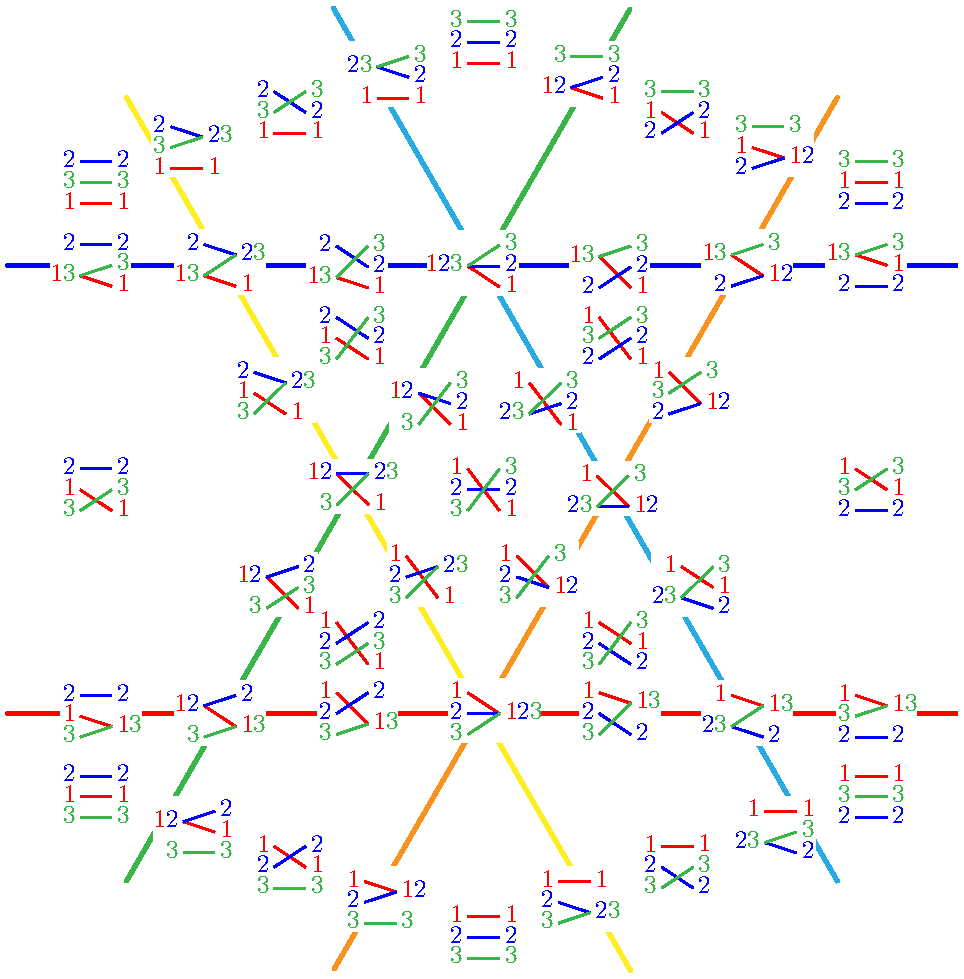
\includegraphics[scale=.9]{B23a}}
	\caption{Labelings of the faces of the arrangement~$\multiBraidArrangement[3][2](\b{a})$ for~$\b{a} = \begin{bmatrix} 0 & 0 \\ -1 & -1 \end{bmatrix}$.}
	\label{fig:B23a}
\end{figure}

\begin{figure}
	\centerline{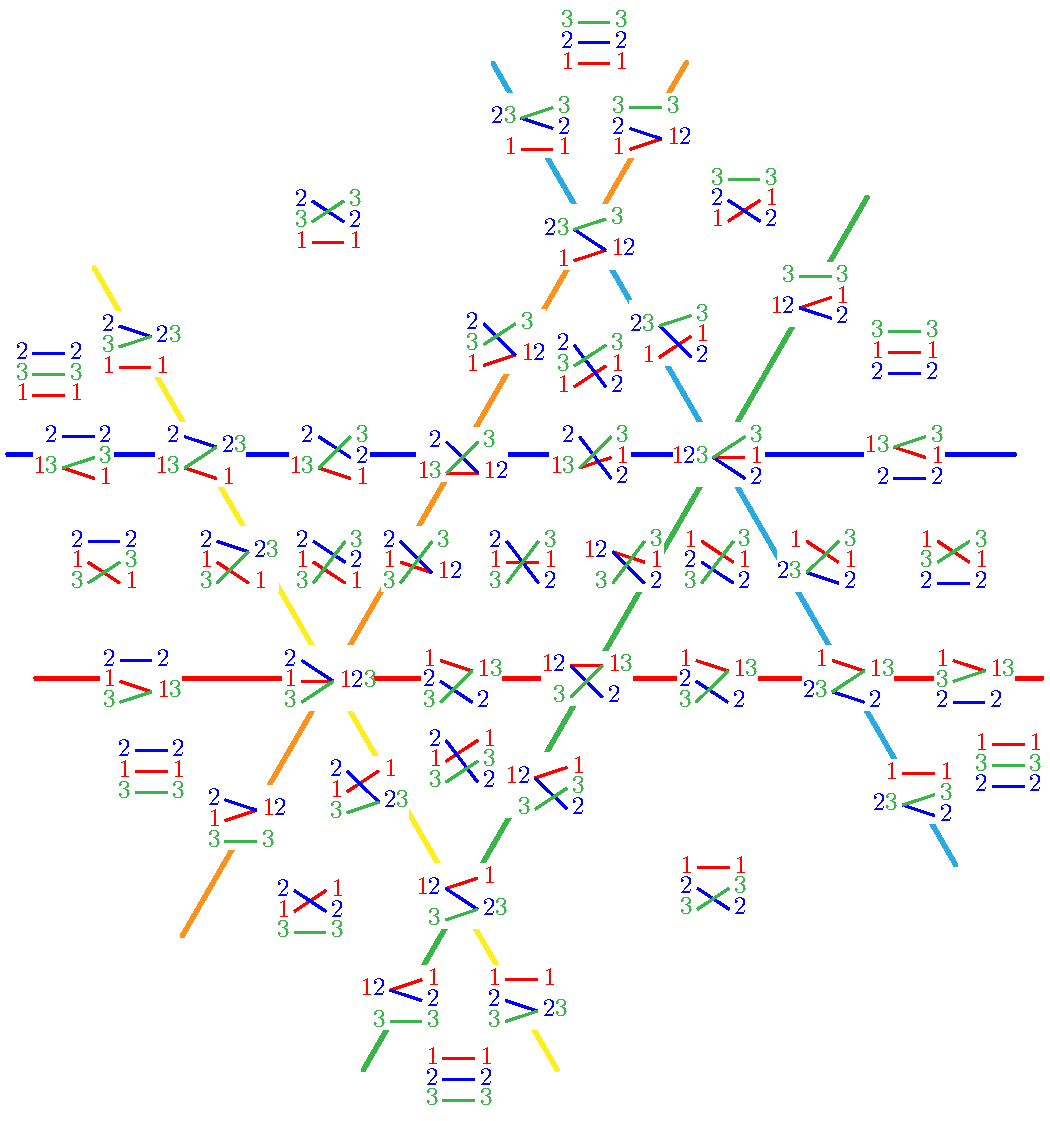
\includegraphics[scale=.9]{B23b}}
	\caption{Labelings of the faces of the arrangement~$\multiBraidArrangement[3][2](\b{a})$ for~$\b{a} = \begin{bmatrix} 0 & 0 \\ 1 & -2 \end{bmatrix}$.}
	\label{fig:B23b}
\end{figure}

We now fix a generic translation matrix~$\b{a} \eqdef (a_{i,j})$ and still denote by~$A_{i,s,t} \eqdef \smash{\sum_{s \le j < t} a_{i,j}}$ for all~$1 \le s < t \le n$ and~$i \in [\ell]$ (and often write~$A_{i,t,s}$ for~$-A_{i,s,t}$).
The objective of this section is to describe
\begin{itemize}
\item the ordered $(\ell,n)$-partitions forests of the upper set~$\orderedForestPoset(\b{a})$ with a given underlying (unordered) $(\ell,n)$-partition forest (\cref{subsec:PFtoOPF}),
\item a criterion to decide whether a given ordered $(\ell,n)$-partition forest belongs to the upper set~$\orderedForestPoset(\b{a})$, \ie corresponds to a face of~$\multiBraidArrangement(\b{a})$ (\cref{subsec:criterionOPF}).
\end{itemize}

%%%%%%%%%%%%%%%

\subsection{From partition forests to ordered partition forests}
\label{subsec:PFtoOPF}

In this section, we describe the ordered $(\ell,n)$-partitions forests~$\order{\b{F}}$ of the upper set~$\orderedForestPoset(\b{a})$ with a given underlying $(\ell,n)$-partition forest~$\b{F}$.
We denote by~$cc(\b{F})$ the connected components of~$\b{F}$, meaning the partition of~$[n]$ given by the hyperedge labels of the connected components of the intersection hypergraph of~$\b{F}$.
We first observe that the choice of~$\b{a}$ fixes the order of the parts in a common connected component of~$\b{F}$.

\begin{proposition}
\label{prop:PFtoOPF1}
Consider a $(\ell,n)$-partition forest~$\b{F} \eqdef (F_1, \dots, F_\ell)$, and two integers~$s,t \in [n]$ labeling two hyperedges in the same connected component of the intersection hypergraph of~$\b{F}$.
Assume that the unique path from~$s$ to~$t$ in the hypergraph of~$\b{F}$ passes through the hyperedges labeled by~$s = r_0, \dots, r_q = t$ and through parts of the partitions~$F_{i_1}, \dots, F_{i_q}$.
Then for any ordered $(\ell,n)$-partition forest~$\order{\b{F}} \eqdef (\order{F_1}, \dots, \order{F_\ell})$ of the upper set~$\orderedForestPoset(\b{a})$ with underlying $(\ell,n)$-partition forest~$\b{F}$ and any~$i \in [\ell]$, the order of~$s$ and~$t$ in~$\order{F}_i$ is given by the sign of~$A_{i,s,t} - \sum_{p \in [q]} A_{i_p, r_{p-1}, r_p}$.
\end{proposition}

\begin{proof}
Consider any point~$\b{x}$ in the face of~$\multiBraidArrangement(\b{a})$ corresponding to~$\order{\b{F}}$.
Along the path from~$s$ to~$t$, we have~$x_{r_{p-1}} - x_{r_p} = A_{i_p, r_{p-1}, r_p}$ for each~$p \in [q]$.
Hence, we obtain that
\[
x_s - x_t = \sum_{p \in [q]}  (x_{r_{p-1}} - x_{r_p}) = \sum_{p \in [q]} A_{i_p, r_{p-1}, r_p}.
\]
The order of~$s,t$ in~$\order{F}_i$ is given by the sign of~$A_{i,s,t} - (x_s - x_t)$, hence of~$A_{i,s,t} - \sum_{p \in [q]} A_{i_p, r_{p-1}, r_p}$.
\end{proof}

We now describe the different ways to order the parts in distinct connected components of~$\b{F}$.
For this, we need the following posets.

\begin{definition}
Consider a $(\ell,n)$-partition forest~$\b{F}$ and denote by~$cc(\b{F})$ the connected components of~$\b{F}$.
For each pair~$s,t \in [n]$ in distinct connected components of~$cc(\b{F})$, we define the chain~$<_{s,t}$ on the $\ell$ triples~$(i,s,t)$ for~$i \in [\ell]$ given by the order of the values~$A_{i,s,t}$.
The \defn{inversion poset}~$\Inv(\b{F}, \b{a})$ is then the poset obtained by quotienting the disjoint union of the chains~$<_{s,t}$ (for all~$s,t \in [n]$ in distinct connected components of~$cc(\b{F})$) by the equivalence relation~$(i,s,t) \equiv (i,s',t')$ if~$s$ and~$s'$ belong to the same part of~$F_i$ and~$t$ and~$t'$ belong to the same part of~$F_i$.
We say that a subset~$X$ of~$\Inv(\b{F}, \b{a})$ is antisymmetric if~$(i,s,t) \in X \iff (i,t,s) \notin X$.
\end{definition}

\begin{proposition}
\label{prop:PFtoOPF2}
The ordered $(\ell,n)$-partition forests of the upper set~$\orderedForestPoset(\b{a})$ with a given underlying $(\ell,n)$-partition forest~$\b{F}$ are in bijection with the antisymmetric lower sets of the inversion poset~$\Inv(\b{F}, \b{a})$.
\end{proposition}

\begin{proof}
Consider an ordered $(\ell,n)$-partition forest~$\order{\b{F}}$ of the upper set~$\orderedForestPoset(\b{a})$.
Let~$\b{x}$ be any point of the face of~$\multiBraidArrangement(\b{a})$ corresponding to~$\order{\b{F}}$.
For each pair~$s,t \in [n]$ in distinct connected components of~$cc(\b{F})$, let~$I_{s,t}(\order{\b{F}})$ be the set of indices~$i \in [\ell]$ such that~$x_s - x_t < A_{i,s,t}$.
Note that~$I_{s,t}$ is by definition a lower set of the chain~$<_{s,t}$ of~$\Inv(\b{F}, \b{a})$.
Hence, $I(\order{F}) \eqdef \bigcup_{s,t} I_{s,t} / {\equiv}$ is a lower set of~$\Inv(\b{F}, \b{a})$.
Moreover, it is clearly antisymmetric since
\[
(i,s,t) \in I(\order{F}) \iff x_s - x_t < A_{i,s,t} \iff x_t - x_s > A_{i,t,s} \iff (i,t,s) \notin I(\order{F}).
\]

Conversely, given an antisymmetric lower set~$I$ of~$\Inv(\b{F}, \b{a})$, we can reconstruct an ordered $(\ell,n)$-partition forest~$\order{\b{F}}$ by ordering each pair~$s,t \in [n]$ in~$\order{F}_i$ 
\begin{itemize}
\item according to \cref{prop:PFtoOPF1} (hence independently of~$I$) if $s$ and~$t$ belong to the same connected component of~$\b{F}$,
\item according to~$I$ if~$s$ and~$t$ belong to distinct connected components of~$\b{F}$. Namely, we place the block of~$\order{F}_i$ containing~$s$ before the block of~$\order{F}_i$ containing~$t$ if and only if~$(i,s,t) \in I$.
\end{itemize}
It is then straightforward to check that the resulting ordered $(\ell,n)$-partition forest belongs to the upper set~$\orderedForestPoset(\b{a})$, by exhibiting a point~$\b{x}$ in of the corresponding face of~$\multiBraidArrangement(\b{a})$.
\end{proof}

%%%%%%%%%%%%%%%

\subsection{A criterion for ordered partition forests}
\label{subsec:criterionOPF}

We now consider a given ordered $(\ell,n)$-partition forest~$\order{F}$ and provide a criterion to decide if it belongs to the upper set~$\orderedForestPoset(\b{a})$ corresponding to the faces of~$\multiBraidArrangement(\b{a})$.
For this, we need the following directed graph associated to~$\order{\b{F}}$.

\begin{definition}
For an ordered partition~$\order{\pi} \eqdef \order{\pi}_1 | \cdots | \order{\pi}_k$ of~$[n]$, we denote by~$D_{\order{\pi}}$ the directed graph on~$[n]$ with an arc~$\max(\order{\pi}_j) \to \min(\order{\pi}_{j+1})$ for each~$j \in [k-1]$ and a cycle~${x_1 \to \dots \to x_p \to x_1}$ for each part~$\order{\pi}_j = \{x_1 < \dots < x_p\}$.
Note that~$D_{\order{\pi}}$ has~$n$ vertices and~$n + k$ arcs.
For an ordered $(\ell,n)$-partition forest~$\order{\b{F}} \eqdef (\order{F_1}, \dots, \order{F_\ell})$, we denote by~$D_{\order{\b{F}}}$ the superposition of the directed graphs~$D_{\order{F}_i}$ for~$i \in [\ell]$, where the arcs of~$D_{\order{F}_i}$ are labeled by~$i$.
\end{definition}

\begin{proposition}
\label{prop:characterizationOPFs}
An ordered $(\ell,n)$-partition forest~$\order{\b{F}}$ belongs to the upper set~$\orderedForestPoset(\b{a})$ if and only if $\sum_{\alpha \in \gamma} A_{i(\alpha), s(\alpha), t(\alpha)} \ge 0$ for any (simple) oriented cycle~$\gamma$ in~$D_{\order{\b{F}}}$, where each arc~$\alpha \in \gamma$ has label~$i(\alpha)$, source~$s(\alpha)$, and target~$t(\alpha)$.
\end{proposition}

\begin{proof}
Consider an ordered $(\ell,n)$-partition forest~$\order{\b{F}} \eqdef (\order{F}_1, \dots, \order{F}_\ell)$.
For each~$i \in [\ell]$, denote by
\begin{itemize}
\item $m_i$ the number of arcs of~$D_{\order{F}_i}$
\item $M_i$ the incidence matrix of~$D_{\order{F}_i}$, with $m_i$ rows and $n$ columns, with a row for each arc~$\alpha$ of~$D_{\order{F}_i}$ containing a $-1$ in column~$s(\alpha)$, a $1$ in column~$t(\alpha)$, and $0$ elsewhere,
\item $\b{z}_i$ the column vector in~$\R^{m_i}$ with a row for each arc~$\alpha$ of~$D_{\order{F}_i}$ containing the value~$A_{i(\alpha), s(\alpha), t(\alpha)}$.
\end{itemize}
Then a point~$\b{x} \in \R^n$ belongs to the face of the $i$\ordinal{} braid arrangement corresponding to~$\order{F}_i$ if and only if it satisfies~$M_i \, \b{x} \le \b{z}_i$.
Hence, $\order{\b{F}}$ appears as a face of the $\b{a}$-braid arrangement if and only if there exists~$\b{x} \in \R^n$ such that~$M \, \b{x} \le \b{z}$, where~$M$ is the $(m \times n)$-matrix (where~$m \eqdef \sum_{i \in [\ell]} m_i$), obtained by piling the matrices~$M_i$ for~$i \in [\ell]$ and similarly, $\b{z}$ is the column vector obtained by piling the vectors~$\b{z}_i$.
A direct application of the Farkas lemma (see \eg \cite[Prop.~1.7]{Ziegler}), there exists~$\b{x} \in \R^n$ such that~$M \, \b{x} \le \b{z}$ if and only if~$\b{c} \b{z} \ge 0$ for any~$\b{c} \in (\R^m)^*$ with~$\b{c} \ge \b{0}$ and~$\b{c} M = \b{0}$.
Now it is classical that the left kernel of the incidence matrix of a directed graph is generated by its circuits (non-necessarily oriented cycles), and that the positive cone in this left kernel is generated by its oriented cycles.
\end{proof}

\begin{remark}
Note that we made some arbitrary choices here by choosing the arc from~$\max(\order{\pi}_j)$ to~$\min(\order{\pi}_{j+1})$ between two consecutive parts~$\order{\pi}_j$ and~$\order{\pi}_{j+1}$ and a cycle inside each part~$\order{\pi}_j$ (while we said that the order in each part is irrelevant).
We could instead have considered all arcs connecting two elements of two consecutive parts, or two elements inside the same part.
Our choices just limit the amount of oriented cycles in~$D_{\order{\pi}}$.
\end{remark}
